\chapter{Détection de contre-exemples et Raffinement}
\section{Fausses alarmes et contre-exemples}


Dans ce chapitre, on s'intéresse aux problèmes que l'on rencontre lors de la vérification de systèmes
où l'ensemble des états atteignables ne peut être calculé que par sur-approximation.

Dans la méthode de vérification basée sur la complétion d'automates d'arbres décrite précédemment
(\textit{cf.} sec.~\ref{sec:completion}), on ne s'est intéressé qu'à la correction de l'approche~:
dans le cas où la vérification réussit, on peut systématiquement  conclure à la préservation
de la propriété. En revanche on ne peut absolument rien conclure lorsque la vérification a échoué.
En effet, à cause de la sur-approximation l'échec peut être dû à une fausse alarme. Les \emph{fausses alarmes} sont
le résultat d'une approximation trop grossière qui contient des états supplémentaires qui n'appartiennent pas au 
système mais violent la propriété. %Et comme ces états n'appartiennent pas au système, le système ne viole pas la propriété.
En pratique, construire une \og bonne \fg\ approximation demande un bon niveau d'expertise du système à vérifier, 
ce qui est d'autant plus difficile lorsque le système est complexe. 
Ainsi, il est rare de trouver immédiatement une approximation qui contienne l'ensemble des états du système et qui en
même temps soit assez fine pour éviter les fausses alarmes. On se propose donc d'améliorer la technique de vérification
pour qu'elle soit plus informative en cas d'échec. En résumé, la propriété peut être violée pour deux raisons~:\\

\begin{itemize}
\item L'exécution du système peut conduire à un état (atteignable) qui ne
  respecte pas la propriété~: l'état constitue un \textbf{contre-exemple}.
  
\item Le système respecte la propriété mais l'approximation trop
  grossière introduit des états (non atteignables) qui violent la
  propriété: c'est une \textbf{fausse alarme}.\\
\end{itemize}


Comme cette méthode de vérification d'une propriété par non-atteignabilité est semi-décidable,
on sait qu'il n'est généralement pas possible de distinguer un contre-exemple d'une fausse alarme,
et donc de savoir si le système viole la propriété.
%% L'enjeu revient donc à chercher si l'intersection contient des états du système. 
%%Alors qu'il est impossible de déterminer si un état quelconque appartient au système,
Cependant on peut repérer les états dont l'appartenance au système est sûre. 
Un tel marquage est réalisable itérativement~: il est sûr de considérer qu'un état
appartient au système si il peut être produit à partir d'un état pour lequel on a aussi l'assurance qu'il
appartient au système. Dualement, on perd l'assurance pour tout état introduit par l'approximation ou
si l'état est obtenu par des transitions issues d'états pour lesquels il n'existe aucune assurance
qu'ils appartiennent au système.
%%%%%%%%%%%%%%%%%%%%% TODO introduire un schéma qui donne les différents cas où l'on sûr ou pas l'on est que des états
%%%%%%%%%%%%%%%%%%%%% appartenant au système ou non.
\begin{figure}[ht!]
  \centering
  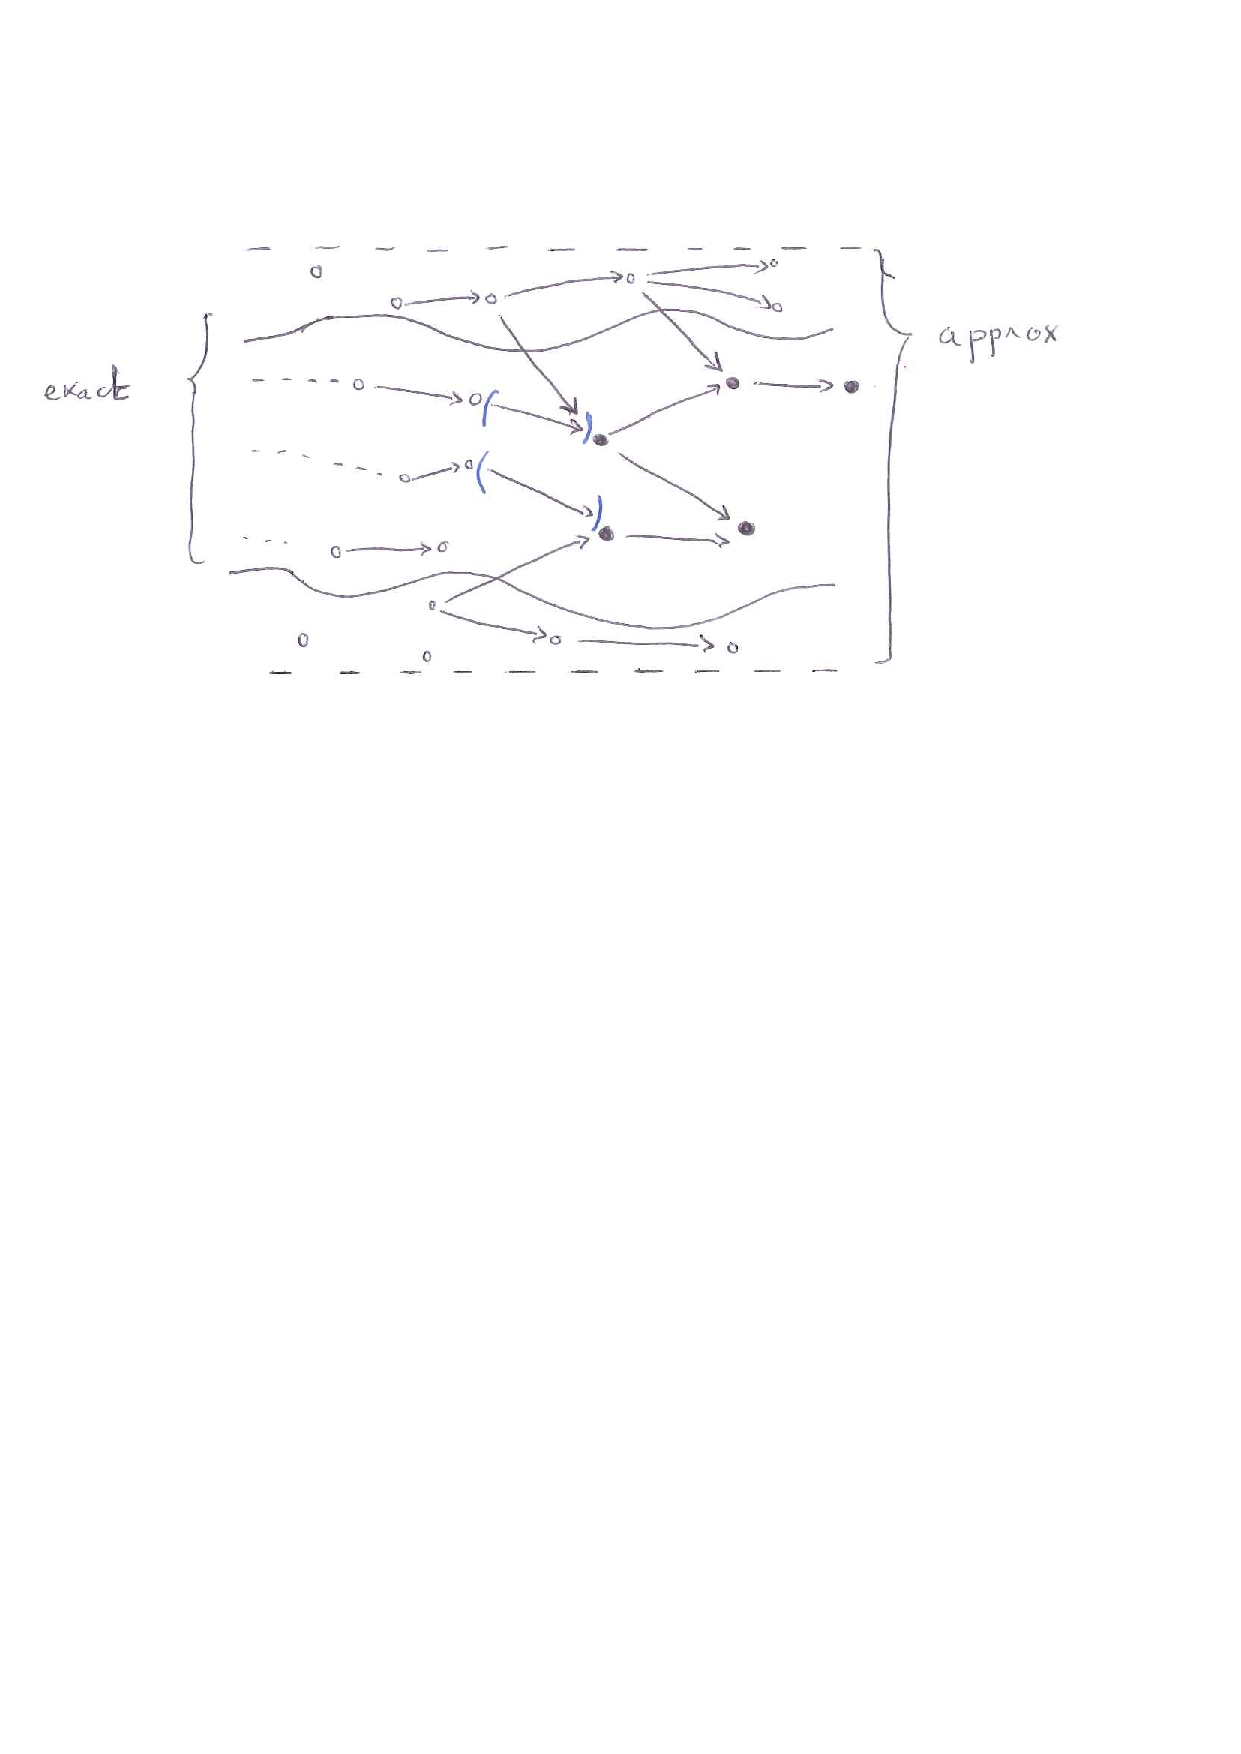
\includegraphics[width=12cm]{4_contre_ex/illustration}
  \caption{\footnotesize }
  \label{fig:illustration}
\end{figure}
Ainsi dans la figure~\ref{fig:illustration}, si les états noirs ont été introduits avant de considérer les transitions
entre parenthèses, on ne peut être sûr que ces états et leur successeurs sont atteignables tant que 
ces transitions n'ont pas été considérées par l'exploration.

Cette technique permet de réduire considérablement la zone d'incertitude en cas d'échec.
Lorsque la vérification de la propriété échoue à cause d'un état $s$ dont on est sûr
qu'il appartienne au système, on peut conclure que le système viole la propriété:
l'état $s$ constitue un \emph{contre-exemple}. Dans le cas contraire on ne sait toujours rien dire,
on est  dans le cas soit d'une fausse alarme soit d'un contre-exemple.

\section{Principe de l'approche à la {CEGAR} appliqué au model-checking régulier}

Il est possible d'améliorer l'approche précédente, en exploitant l'information
lorsque la vérification échoue et que l'on ne peut pas conclure à un contre-exemple ou une fausse alarme.
En effet, si l'on n'est pas sûr qu'un état $s_?$ est atteignable, alors il a été introduit par une étape d'accélération.
Pour cet état $s_?$, on peut envisager les deux situations suivantes:
% En fonction de la réelle nature de chaque état supprimé on peut différencier
% deux cas possibles~:

\begin{itemize}
\item
  Soit $s_?$ n'est pas réellement atteignable: raffiner l'approximation de façon
  à supprimer $s_?$ est correct, puisqu'il s'agit d'une fausse alarme.
\item
  Soit $s_?$ est atteignable: il existe au moins une exécution du système qui passe par cet état~:
  cela signifie que la trace d'exécution qui permet d'atteindre $s_?$ n'a pas encore été considérée
  lors du calcul et qu'une étape d'accélération a introduit l'état $s_?$.
  Même si on retire $s_?$ de l'approximation, comme il est atteignable, on finira toujours
  par produire le terme par des étapes de calcul exact. 
\end{itemize}
On peut donc envisager de supprimer l'état $s_?$ de l'approximation, si l'on tente de compléter à nouveau
l'ensemble des états atteignables. C'est le principe de l'approche à la {CEGAR}
(\emph{Counter-Example Guided Abstraction Refinement})~\cite{DBLP:conf/time/Clarke03}: on retire successivement tous les
états $s_?$ qui conduisent à la mise en échec de la propriété s'il n'est pas possible
de déterminer s'ils sont des contre-exemples ou non. Chaque phase de raffinement conduit 
alors à la reprise du calcul de l'ensemble des atteignables privé des états $s_?$.
Cependant, raffiner l'approximation de l'ensemble des états peut entraîner une divergence du calcul
puisque le raffinement affaiblit l'approximation~: cela impose de raffiner avec parcimonie, pour
éviter d'accroître ce risque de divergence.


Dans~\cite{DBLP:conf/cav/BouajjaniHV04}, Bouajjani et al. ont introduit les premières
techniques à la CEGAR pour le model-checking régulier, avant de
l'étendre aux termes dans~\cite{BouajjaniHRV-Infinity06,BouajjaniHRV-SAS06}. 
Le principe de ces travaux repose sur une pile qui contient tous les automates d'arbres
intermédiaires produits par le calcul depuis l'automate initial.
La relation de transition est définie par $T$ un transducteur d'automates
d'arbres~\cite{TATA}. L'abstraction est construite en utilisant des prédicats 
qui paramètrent les étapes d'accélération.
Les prédicats sont représentés par des automates d'arbres.

Le processus de calcul est basé sur l'alternance étape de transduction
suivie d'une étape d'abstraction. Pour déterminer si un terme
est un contre-exemple ou un terme suspicieux\footnote{\footnotesize un terme dont on ne peut
déterminer si il est atteignable ou non}, l'approche repose sur un
calcul arrière qui impose de construire la relation de transition
inverse $T^{-1}$. À partir d'un ensemble $X_n$ de termes reconnus dans l'automate $M_n$ tels que $X_n$
viole une certaine propriété, on cherche dans les automates précédents quels termes ont permis par $T$
de produire les termes de $X_n$. Pour cela, on calcule un sur-ensemble des prédécesseurs possibles, 
et on recherche ceux qui étaient effectivement reconnus par l'automate $M_{n-1}$, (calcul d'intersection)
ce qui constitue l'ensemble de termes $X_{n-1}$. On recommence le processus jusqu'à:
\begin{itemize}
\item obtenir l'ensemble $X_0 \not= \emptyset$ dont l'un des termes est reconnu par l'automate initial,
  permet de produire l'un des termes de $X_n$: l'ensemble  $X_n$ contient un contre-exemple.

\item obtenir $X^k = \emptyset$ pour $k \le n$, on peut alors en déduire 
  que les termes de $X_{k+1}$ n'ont pas été produits par l'application du transducteur $T$ sur l'automate $M_k$.
  Ils sont donc le résultat d'une étape d'accélération réalisée sur l'automate $M_{k+1}$.
  Donc pour éviter les termes $M_n$, il faut retirer les termes de $M_{k+1}$ qui sont
  à l'origine de leur introduction en raffinant l'abstraction réalisée sur $M_{k+1}$.
\end{itemize}
Cette opération est d'autant plus coûteuse que la propriété est violée tardivement. 
Plus $n$ est grand, plus la recherche en arrière coûte cher, les opérations booléennes sur
les automates d'arbres ayant un coût non négligeable.


\begin{figure}[ht!]
  \centering
  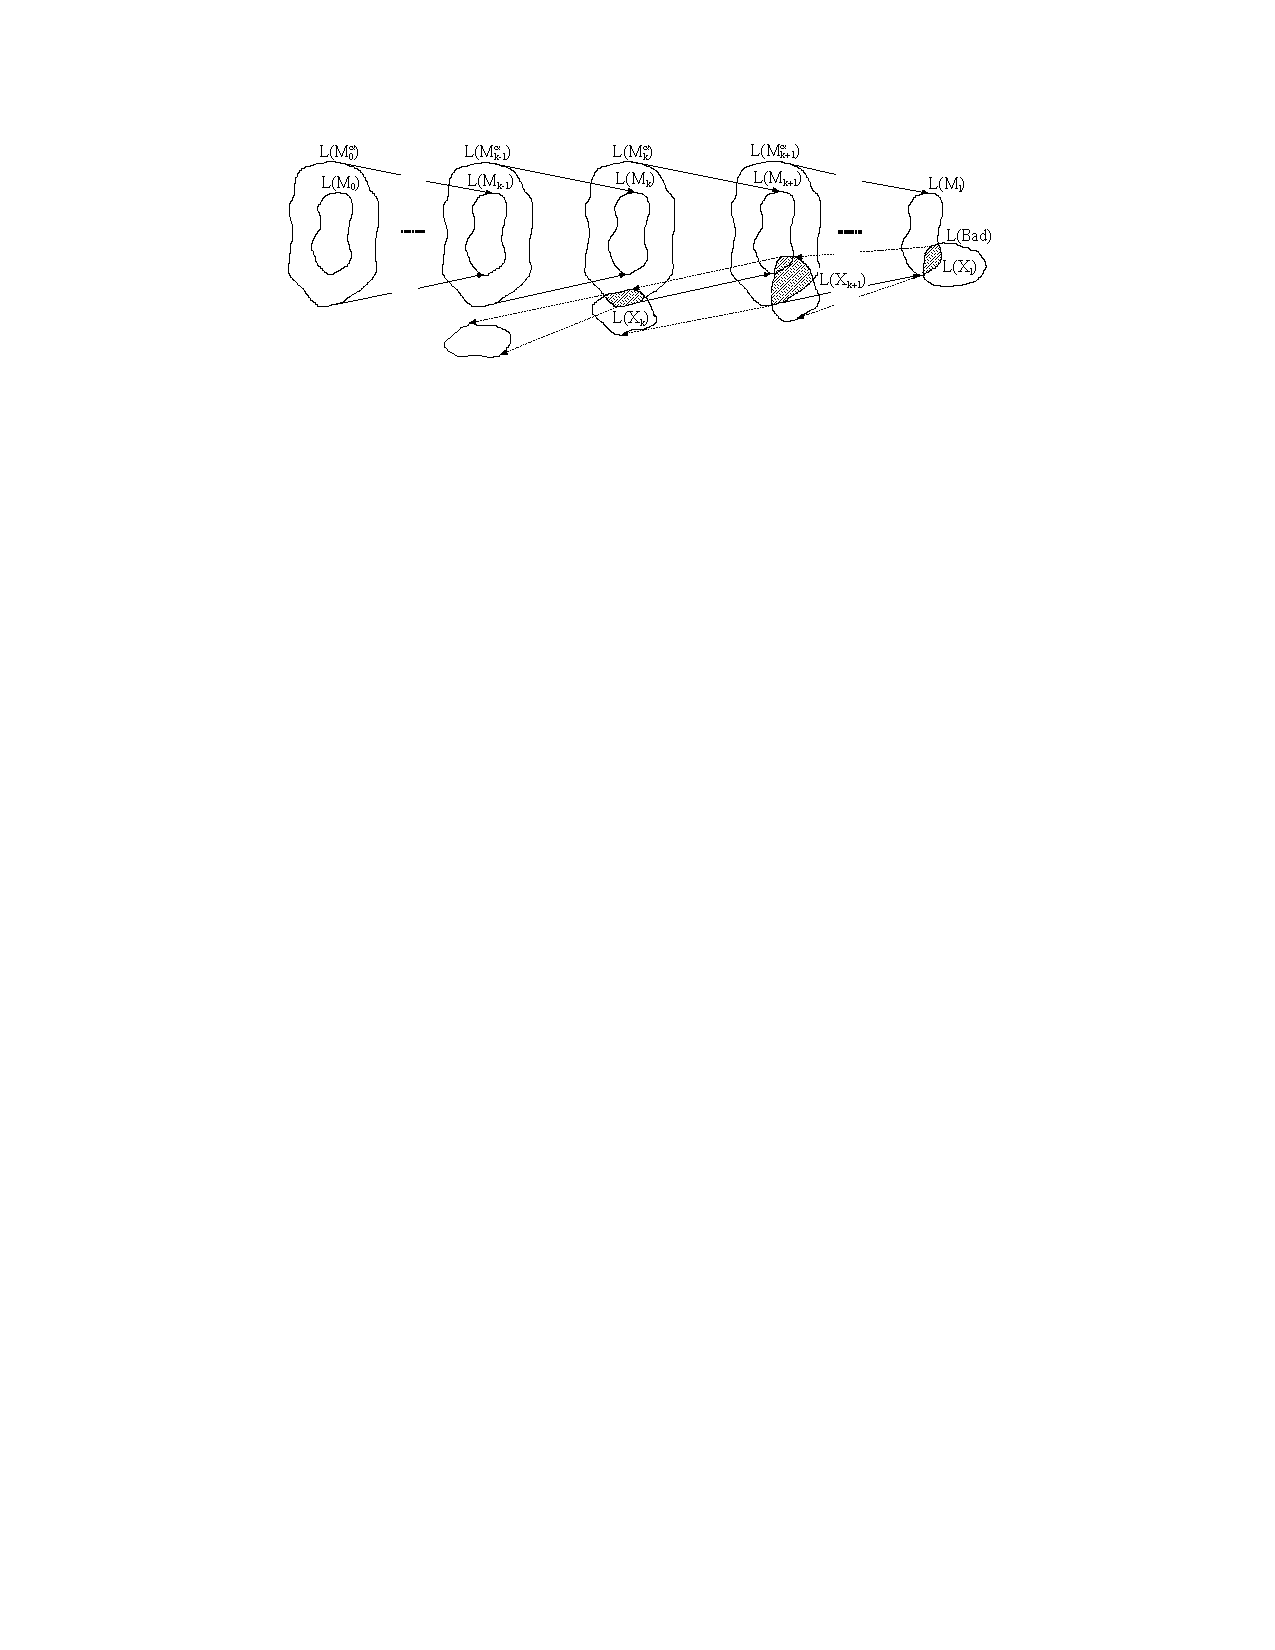
\includegraphics[width=14cm]{4_contre_ex/armc}
  \caption{\footnotesize Le calcul en arrière en model-checking régulier (fig. extraite de~\cite{DBLP:conf/cav/BouajjaniHV04})}
\end{figure}

Dans~\cite{BCHK08}, Boichut et al. ont tenté une approche similaire mais en utilisant des
règles de réécriture à la place des transducteurs et définissent l'abstraction des règles d'approximation
directement pour l'automate. De la même manière, le processus est basé sur la sauvegarde des automates
obtenus à chaque pas de calcul. Néanmoins, cette technique nécessite
que les règles de réécriture soient linéaires à gauche et à droite, pour effectuer le
calcul en arrière: la complétion d'automates d'arbres nécessite de
modéliser la relation de transition $Rel$ par un système de réécriture
linéaire à gauche, et le calcul arrière -- lui aussi réalisé par la
complétion -- nécessite la relation $Rel^{-1}$ définie en retournant
chaque règle $l \rw r \in \R$ en $r \rw l \in \R^{-1}$, imposant aux
membres droits dans $\R$ d'être linéaires.  Si la modélisation de
systèmes par un ensemble de règles de réécriture linéaires est
toujours possible, elle peut s'avérer moins immédiate qu'avec
des règles de réécritures linéaires à gauches.


%%%%%%%%%%%%%%%%%%%%%%%%%%%%%%%%%%%%%%%%%%%%%%%%%%%%%%%%%%%%%%%%%%%%%%%%%%%%%%%%%%%%%%%
%%%%%%%%%%%%%%%%%%%% VERSION EXTRAITE DE ../plan/plan_contre_ex.mm %%%%%%%%%%%%%%%%%%%%
%%%%%%%%%%%%%%%%%%%%%%%%%%%%%%%%%%%%%%%%%%%%%%%%%%%%%%%%%%%%%%%%%%%%%%%%%%%%%%%%%%%%%%%

\section{Contre-exemples et automates d'arbres}

% {Bouajjani \cite{artmc06}, Besançon \cite{fib:arra08}}
% {Approches intéressantes, mais limitées d'un point de vue complexité et expressivité}
% {Utilisation de l'inclusion d'automates d'arbres + intersection, systèmes linéaires à droite et
%   à gauche : ça n'est pas le cas du TRS de Java (non linéaire à droite) (pour éviter les calculs d'inclusion, calcul en arrière à partir de la propriété)}
% {Autres approches ? voir les papiers de Besançon ???}
%\bigskip
La contribution de ce chapitre est de proposer une solution pour améliorer
la complétion en cas d'échec et de proposer une procédure de raffinement
à la CEGAR pour l'algorithme de complétion d'automates d'arbres sans avoir recours 
au calcul en arrière pour déterminer si un terme est un contre-exemple ou non.
On espère ainsi gagner en performance par rapport aux techniques existantes.
Pour cela, on définit des automates d'arbres instrumentés que
l'on appelle \textbf{$\RE$-automates} et dont la sémantique 
nous informe sur la manière de réécrire les termes.
En résumé l'automate caractérise les termes ajoutés par réécriture
de $\R$ ou par réécriture de $\R$ modulo $E$ en gardant une trace
des équations utilisées pendant l'accélération.
On propose alors une procédure de complétion d'un $\RE$-automate
pour $\R$ un système de règles linéaires à gauche et un ensemble d'équations $E$.
L'information nécessaire étant maintenue à jour dans le $\RE$-automate courant, 
il n'est plus nécessaire de revenir sur les calculs antérieurs pour
connaître la nature d'un terme: l'exécution de l'automate pour un terme $t$
permet d'obtenir des informations sur l'atteignabilité. L'automate constitue en lui-même
la procédure de semi-décision.
Pour un terme $t$ reconnu par le $\RE$-automate, la sémantique informe des différentes étapes
d'accélération qui ont été nécessaire à sa construction. Lorsque l'automate indique qu'il n'y a
pas eu d'abstraction pour obtenir $t$, le terme est atteignable par $\R$.  Dans le cas
contraire, on dispose de l'information nécessaire pour raffiner efficacement l'approximation par la procédure 
d'élagage du $\RE$-automate que l'on propose.
De plus, nous verrons que la technique de raffinement développée ici est plus
précise que celle présentée dans~\cite{BCHK08}, ce qui lui permet  
converger plus fréquemment. Enfin, ce travail étend les abstractions
équationnelles~\cite{MeseguerPM-TCS08,Takai-RTA04} pour la détection
de contre-exemples et le raffinement.

%%Our approach is naturally more efficient than the one of
%%Bouajjani et al. as it does not require to store the intermediary
%%computation steps and apply a reverse of the transition relation to
%%conclude whether the term is reachable or not.

%\paragraph{Related work.} 



\section{L'intuition initiale}
\label{sec:intuition}
L'idée qui a conduit à la l'introduction des $\RE$-automates peut être illustrée à l'aide de l'exemple~\ref{ex:intuition}.
\begin{example}
  \label{ex:intuition}
  Soit $\A$ un automate défini comme:
  \begin{itemize}
  \item $\Q_f = \{ q_g, q_f\}$
  \item $\Delta = \{ f(q_a) \rw q_f,\ g(q_b) \rw q_g,\ a\rw q_a,\ b\rw q_b\}$
  \end{itemize}
  L'automate reconnaît les termes $f(a)$ et $g(b)$.
  On applique à cet automate l'équation $a = b$ ce qui permet de fusionner les états $q_a$ et $q_b$
  \[\xymatrix{
    a \ar@{=}_{E}[r]\ar[d]_{\A}^{*} & b \ar[d]_{*}^{\A}\\
    q_a & q_b
  }
  \]
  On obtient l'automate $\A'$ formé par les transitions $\Delta' = \{ f(q_a) \rw q_f,\ g(q_a) \rw q_g,\ a\rw q_a,\ b\rw q_a\}$
  où $q_b$ est remplacé par $q_a$. Ainsi les termes $a$ et $b$ sont dans la même classe d'équivalence, ce qui a pour 
  conséquence d'ajouter les termes $f(b) \in \Lang(\A', q_f)$, et $g(a) \in \Lang(\A', q_g)$.
\end{example}

  La fusion produit bien l'effet escompté sur le langage reconnu. En revanche, lorsque l'on se place du point de vue
  de l'état $q_f$, la fusion ne permet pas de comprendre à posteriori que  $f(b)$ est obtenu par l'abstraction, 
  alors que $f(a)$ était déjà reconnu par $\A$. Dualement, on peut remarquer le même problème à l'état $q_g$ avec les termes
  $g(b)$ et $g(a)$.

  Une manière de pallier à cette limitation consiste à rendre explicites les opérations de fusion.
  La solution retenue consiste à remplacer le renommage par des $\varepsilon$-transitions particulières:
  \[\xymatrix{
    a \ar@{=}_{E}[r]\ar[d]_{\A}^{*} & b \ar[d]_{*}^{\A}\\
    q_a \ar@/^0.6pc/[r]^{=} & q_b \ar@/^0.6pc/[l]^{=}
  }
  \]
  Maintenant, on peut savoir si un terme a été ajouté au langage grâce à l'abstraction ou non, juste en considérant
  les transitions utilisées pour le reconnaître:

  \begin{example}
    \begin{description}
    \item $f(a) \lrw f(q_a) \lrw q_f$ indique $f(a)$ ne vient pas de l'abstraction,

    \item $f(b) \lrw f(q_b) \mathbf{\stackrel{=}{\lrw}} f(q_a) \lrw q_f$ est obtenu par l'abstraction.
    \end{description}
  \end{example}
  
  Cela est suffisant pour caractériser la relation de causalité liée
  aux étapes d'abstraction qui peuvent avoir lieu lors de la
  complétion de l'automate.  C'est sur ce principe que repose les
  $\RE$-automates introduits dans la section~\ref{sec:RE-automaton}.



\section{Définition d'un $\RE$-automate}
\label{sec:RE-automaton}

Un $\RE$-automate est une extension de la définition standard des automates d'arbres,
dont la sémantique donne des informations sur les termes reconnus par cet automate
notamment pour un problème d'atteignabilité. Elle permet en particulier 
de distinguer les termes pour lesquels l'atteignabilité est sûre des autres termes.
Définir un $\RE$-automate n'a donc de sens que dans le cadre d'un problème d'atteignabilité 
donné $(I, \R, Bad)$ et d'une abstraction définie par un ensemble $E$ d'équations. 
On notera que le cas particulier du calcul exact
dénoté par $E = \emptyset$ est couvert par l'approche, mais ne se révèle pas intéressant puisque
le problème soulevé n'existe que dans le cas d'une sur-approximation.

Soit un problème d'atteignabilité défini dans l'ensemble de termes $\TF$ avec 
$I$ comme ensemble fini de termes initiaux $\R$ un ensemble de règles de réécriture
et $E$ un ensemble d'équations.

% $\Deq$ denotes a subset
% of the equivalence relation induced by the set of equations.
% Moreover, we will be able to know that a term recognized using a
% transition of $\Deq$ is the result of a widening step.  The
% example~\ref{ex:semantics} illustrates the principle of a
% $\RE$-Automaton.


%We now give the formal definition for $\RE$-automata.

\begin{definition}
  \label{def:re-automaton}
  Un \textbf{$\RE$-Automate} est un automate d'arbres défini comme un quadruplet de la forme
  $\A= \langle \F, \Q, \Q_f,\Delta \cup \Drw \cup \Deq\rangle$,
  avec $\Q_f \subseteq \Q$ et composé de 3 ensembles de transitions distinctes~:

  \begin{description}
  \item $\Delta$ est un ensemble de transitions normalisées (\textit{c.f.} définition~\ref{def:transitions}),
  \item $\Deq$ est un ensemble de $\varepsilon$-transitions,
  \item $\Drw$ est un ensemble de 
  $\varepsilon$-transitions étiquetées par $\top$ ou par une conjonction de prédicats de la forme $Eq(q, q')$ 
  avec $q, q' \in \Q$, et $q \rw q' \in \Deq$.
  \end{description}
\end{definition}


Un $\RE$-automate est un automate d'arbre dans lequel les transitions sont classées en trois catégories.  D'une part les
transitions normalisées et deux ensembles distincts de $\varepsilon$-transitions~:
\begin{itemize}
\item les premières caractérisent la relation de réécriture qui peut exister entre les classes
  d'équivalence de l'automate, comme les $\varepsilon$-transitions produites par la complétion~\ref{sec:completion}, 
  mais étiquetées par des formules logiques.

\item les secondes définissent la relation d'abstraction qui peut exister entre deux classes d'équivalence comme illustré en 
  section~\ref{sec:intuition}.
\end{itemize}

% Comme pour les $\R$-automates, la sémantique d'un $\RE$-automate n'a de sens que dans le contexte d'un problème d'atteignabilité
% constitué d'un ensemble initial, d'un système de réécriture, et d'un ensemble d'équations
% \footnote{\footnotesize l'ensemble des équations peut être éventuellement vide, mais on se ramène alors au cas du calcul 
%   sans approximation couvert par les $\R$-automates.}.


\begin{example}
  \label{ex:semantics}
  Soit $\A$ un $\RE$-automate reconnaissant dans l'état final $\mathbf{q_f}$
  le système $(\F, I, \R)$ défini par 

  $I = f(a)$, $\R = \{f(c) \rw g(c),\ a \rw b\}$, et un ensemble d'équations $E = \{ b = c\}$.

  Dans $\A$, l'égalité $b = c$ est symbolisée par les 2 transitions $q_c
  \rw q_b$ et $q_b \rw q_c$ de $\Deq$, en tenant compte que $b$ et $c$
  sont respectivement reconnus dans les états $q_b$ et $q_c$.
  
  Ainsi du point de vue de l'état $q_c$, la transition $q_b \rw q_c$
  nous indique que le terme $b$ est obtenu à partir du terme $c$ par égalité.
  On peut constater que la transition $q_c \rw q_b$ nous permet 
  de conclure réciproquement que le terme $c$ est obtenu à partir du terme $b$.

  Les transitions $q_g \rw q_f$ et $q_b \rw q_a$ dénotent des étapes de réécriture.
  De la même manière que pour les transitions qui dénotent l'équation $b=c$, du point
  de vue de l'état $q_a$, la transition $q_b \rw q_a$ permet de déduire que le terme
  $b$ est un descendant par $\RE$ du terme $a$. La transition $q_g \rw q_f$ indique 
  aussi à l'état $q_f$ que le $g(c)$ est un descendant de $f(a)$ par $\RE$.

  Les deux transitions $q_g \rw q_f$ et $q_b \rw q_a$ permettent de déduire que l'on a $f(a) \rw^*_\RE g(c)$
  et $a \rw^*_\RE b$. En revanche, lorsqu'on déplie la relation $f(a) \rw^*_\RE g(c)$, on obtient la chaîne
  $f(a) \rw_\R f(b) =_E f(c) \rw_\R g(c)$, qui utilise l'égalité $b = c$ pour passer de $g(b)$ à $g(c)$, relation que l'on peut 
  déduire de la transition $q_c \rw q_b$. Ainsi, on étiquette la transition $q_g \rw q_f$
  avec la formule $Eq(q_c, q_b)$ pour reporter cette information. 
  D'autre part, la transition $q_b \rw q_a$ est étiquetée avec $\top$ ce qui signifie 
  qu'aucune égalité n'est utilisée pour réécrire $a$ en $b$: de cette transition, on déduit $a \rw^*_\R b$.
  \begin{center}
    %\centering
    \tikz[thick, scale=1]{
      \node (qf) at (0, 0)   {$\mathbf{q_f}$};
      \node (qg) at (4, 0)   {$q_g$};
      \node (f)  at (0,-1.5) {$f(\;q_a\;)$};
      \node (g)  at (4,-1.5) {$g(\;q_c\;)$};
      \node (qa) at (0,-2.8) {$q_a$};
      \node (qb) at (2,-2.8) {$q_b$};
      \node (qc) at (4,-2.8) {$q_c$};
      \node (a)  at (0,-4.3) {$a$};
      \node (b)  at (2,-4.3) {$b$};
      \node (c)  at (4,-4.3) {$c$};
      % \Delta
      \draw [->] (f) edge (qf);
      \draw [->] (g) edge (qg);
      \draw [->] (a) edge (qa);
      \draw [->] (b) edge (qb);
      \draw [->] (c) edge (qc);
      % liens de descendance
      \draw [dashed] (f) edge (qa);
      \draw [dashed] (g) edge (qc);
      % \Drw
      \draw [->, bend right=15] (qg) to node[auto, swap] {\footnotesize$Eq(q_c, q_b)$} (qf);
      \draw [->, bend right=15] (qb) to node[auto, swap] {\footnotesize$\top$} (qa);
      % \Deq
      \draw [->, bend right=15] (qb) to node[auto, swap] {\footnotesize$=$} (qc);
      \draw [->, bend right=15] (qc) to node[auto, swap] {\footnotesize$=$} (qb);
    }
  \end{center}
  %\caption{Example of $\RE$-automaton}
\end{example}

%%% Local Variables: 
%%% mode: latex
%%% TeX-master: "../main"
%%% TeX-PDF-mode: t
%%% End:



% Les $\RE$-automates sont une extension des $\R$-automates introduits dans
% \cite{BoyerG-RULE09}. 

Intuitivement, dans un $\RE$-automate, les termes sont reconnus en utilisant les transitions de $\Delta$, les transitions de $\Drw$ dénotent la relation de réécriture
entre ces termes, et les $\varepsilon$-transitions de $\Deq$ dénotent
les étapes d'abstraction. Chaque transition de $\Drw$ est étiquetée par une formule logique
correspondant aux approximations réalisées pour produire l'étape de réécriture. 
Plus exactement, la formule indique quelles sont les étapes d'abstraction qui ont été nécessaires 
pour produire le terme qui a pu être réécrit. 
% Plus exactement, 
% La relation caractérisée est semblable à celle dénotées par les automates obtenus par la complétion:
Ainsi, lorsque la formule est $\top$, aucune approximation n'est nécessaire et le terme
est atteignable simplement par réécriture, sinon le terme a été produit par réécriture 
modulo $E$. Dans~\cite{GenetR-JSC10}, les auteurs établissent déjà le lien entre la réécriture $\RE$
et les automates produit par la complétion.


%\comments{Sinon, si la formule n'est pas équivalente à $\top$, th}


\subsection{Sémantique}


% We introduce $\f^=$ which denotes the transitive closure of transitions of $\Delta \cup \Deq$.
% The couple $(Q, \f^=)$ induces the equivalence relation such that if terms $u$ and $v$
% are in the same equivalence classe, then $u =_E v$.

%%%%%%%%%%%%%%%%%%% FSTTCS %%%%%%%%%%%%%%%%%%%%%%%%


%\comments{On s'en sert?: In the following, we assume that logical
%formulas are always transformed into an equivalent \emph{Disjunctive Normal
%  Form} using standard logic equivalences.} \noindent 
%%Normalized transitions of $\Delta$ in a $\RE$-automaton recognize terms, called
%%{\em representative}, whereas $\varepsilon$-transitions represent rewriting and
%%equivalence relations between them. 

%%\comments{Axel: shall we keep the definition of sets of representative?}

Dans la suite, on utilisera $\rw_\Delta^*$ pour dénoter la clôture transitive et réflexive de 
la relation $\rw_\Delta$ induite par tout ensemble $\Delta$ de transitions. 
Dans le cas où $\Delta$ est l'ensemble de toutes les transitions normalisées on utilisera $\rwne$ 
pour $\rw_\Delta$, et $\rwne^*$ pour $\rw^*_\Delta$.
Pour $\Delta$ un ensemble donné de transitions normalisées d'un $\RE$-automate, 
on définit l'ensemble des représentants d'un état comme $\Rep(q) = \{ t \in \TF | t \rwne^* q\}$. 
On introduit maintenant la définition formelle des exécutions d'un $\RE$-automate.

%This $\rwned$ is a particular case of the new rewriting relation $\xrw{\alpha}_\A$
%of $\RE$-automata. 

\begin{definition}
  \label{def:xrw_alpha}
  On définit un pas d'\textbf{exécution du $\RE$-automate} $\A$ sur le terme $t \in \TFQ$ reconnu en l'état $q$ 
  par la relation $t \xrw{\alpha}_\A q$ définie comme:
  \begin{itemize}
  \item $t|_p = f(q_1, \dots, q_n)$ et $f(q_1, \dots, q_n) \rw q \in \Delta$
    alors $t \xrw{\top}_\A t[q]_p$
  \item $t|_p = q$ et $q \rw q' \in \Deq$ alors $t \xrw{Eq(q, q')}_\A t[q']_p$
  \item $t|_p = q$ et $q \xrw{\alpha} q' \in \Drw$ alors $t \xrw{\alpha}_\A t[q']_p$ 
%     where $\alpha = \left\{
%       \begin{array}{ll}
%         \alpha_k &\textrm{if } 1 \le k \le n \land \phi = \bigvee_1^n \alpha_i\\
%         \top &  \textrm{if } \phi = \top
%       \end{array}\right.
%     $
  \end{itemize}
  On définit de manière plus générale l'exécution du $\RE$-automate $\A$ comme la clôture 
  transitive et réflexive de $\xrw{\alpha}_\A$:
  \begin{itemize}
  \item $t \xrw{\top}_\A^* t$
  \item $t \xrw{\alpha}_\A v$ alors $t \xrw{\alpha}^*_\A v$
  \item $t \xrw{\alpha}_\A t'$ et  $t' \xrw{\alpha'}_\A t''$ alors $t \xrw{\alpha \land \alpha'}_\A t''$
  \end{itemize}
\end{definition}

\noindent
Une exécution $\xrw{\alpha}^*$ abstrait une séquence de réécriture de $\rwmod$. Si $t
\xrw{\alpha}^* q$, alors il existe un terme $s\in \Rep(q)$ tel que 
$s\rwmod^* t$. La formule $\alpha$ dénote le sous-ensemble de transitions de $\Deq$ 
utilisées pour reconnaître $t$ dans $q$.


%%i.e. the equivalence
%%steps, induced by $E$, needed to rewrite $s$ into $t$ using
%%$\rwmod$.
\begin{example}
  On considère le $\RE$-automate $\A$ de l'exemple~\ref{ex:semantics}, puis l'exécution
  $g(b) \xrw{Eq(q_b, q_c) \land Eq (q_c, q_b)}^*_\A q_f$ qui permet à $\A$ de reconnaître le terme $g(b)$.
  on sait qu'il existe une séquence de réécriture $\rwmod$ à partir de $f(a)$, l'unique terme
  de l'ensemble des représentants de $Rep(q)$, pour produire $g(b)$. 
  La formule indique que cette séquence de réécriture utilise 
  la relation d'équivalence  induite par $b = c$ dans les deux sens
  (transitions $q_b \rw q_c$ et $q_c \rw q_b$).
\end{example}


La relation $\xrw{\alpha}^*$ correspond à la relation standard de réécriture 
(\textit{c.f.} la section~\ref{sec:automates}) d'un automate d'arbres instrumenté avec
des formules logiques.

\begin{theorem}\label{th:equiv}{\quad\quad
  $\forall t\in\TFQ,\; q \in \Q,\; (\exists \alpha\; t \xrw{\alpha}^*_\A q) \equ t \rw_\A^* q$}
\end{theorem}

\begin{proof}
  La preuve est simple et peut se réaliser par induction en montrant qu'il suffit
  d'ignorer les formules qui sont manipulées par la définition~\ref{def:xrw_alpha},
  pour retrouver la relation originale $\rw_\A^*$. 
\end{proof}

Ce théorème est rassurant puisque les $\RE$-automates ont la même expressivité
que les automates d'arbres, ce qui permet de rester dans la classe des langages réguliers
de termes. Ce point est important puisqu'on ne perd pas d'expressivité pour représenter les
approximations. D'autre part, puisqu'on ne gagne pas en expressivité
non plus, on évite le coût du passage à des classes de langages non réguliers
comme c'est le cas par exemple pour des automates à contraintes~\cite{TATA}.


On s'intéresse maintenant aux $\RE$-automates {\em bien définis}. 
La propriété de bonne définition permet d'assurer que l'information
qu'apporte les $\RE$-automates est correcte par rapport à la réécriture
par $\R$ et $E$. La propriété de bonne définition est nécessaire pour s'assurer 
lors du raffinement que l'on distinguera correctement les contre-exemples des faux-positifs.

% \comments{plus précis que la relation de $\RE$-cohérence, et sera simplement admise dans ce chapitre...}

\begin{definition}[Un $\RE$-automate bien défini]
  \label{def:well-defined}
  $\A$ est un $\RE$-automate \emph{bien défini}, si :
  % The second point of the definition is used to refine the $\RE$-automaton: a rewriting step of $\rwmod$
  % denoted by $q \xrw{\phi} q'$ holds thanks to the subset of transitions of $\Deq$
  % occurring in $\phi$. If we remove the transitions of $\Deq$ such that $\phi$
  % does not hold, then the transition $q \xrw{\phi} q'$ disappears and the term is 
  % no longer recognized.
  \begin{itemize}
  \item Pour tout état $q$ de $\A$, et tout terme $v$ tel que
    $v \xrw{\top}^*_\A q$, il existe $u$ un représentant de l'état $q$ tel que $u \rw^*_\R v$
  \item Si $q \xrw{\phi} q'$ est une transition de $\Drw$, alors il existe deux termes
    $s,t\in \TF$ tels que $s\xrw{\phi}^*_\A q$, $t\xrw{\top}^*_\A q'$
    et $t \rw_\R s$.
  \end{itemize}
\end{definition}

\noindent
Le premier point de la définition~\ref{def:well-defined} assure que
tout terme reconnu en utilisant uniquement des transitions étiquetées
par la formule $\top$ est atteignable à partir de l'ensemble initial.
Le second point est utilisé pour raffiner l'automate. Une séquence de réécriture
$\rwmod$ dénotée par $q \xrw{\phi} q'$ est possible grâce à certaines transitions
de $\Deq$ caractérisées par $\phi$. Si on supprime ces transitions de $\Deq$ de telle sorte
que $\phi$ devienne fausse, alors la transition $q \xrw{\phi} q'$ sera aussi supprimée.

A partir de cette définition, un terme $t$ qui est reconnu en 
utilisant au moins une transition étiquetée avec une formule différente de $\top$
peut être enlevée du $\RE$-automate en supprimant des transitions de $\Deq$.
Cette opération d'``élagage''  est illustrée ci-dessous.

\begin{example}
  \label{ex:pruning}
  On reprend le $\RE$-automate $\A$ de l'exemple~\ref{ex:semantics}.
  Cet automate reconnaît le terme $g(c)$. En effet, d'après la
  définition~\ref{def:xrw_alpha}, on a $g(c) \xrw{Eq(q_c, q_b)}_\A^* q_f$. On considère maintenant la séquence de réécriture $f(a) \rw_\R f(b) =_E f(c) 
  \rw_\R g(c)$. On peut voir que si l'étape $f(b) =_E f(c)$ dénotée par la 
  transition $q_c \rw q_b$ est supprimée, alors $g(c)$ devient non-atteignable. 
  La première étape de l'élagage de $\A$ consiste donc à retirer cette
  transition. Dans un deuxième temps, on propage cette information en retirant
  toutes les transitions de $\Drw$ étiquetées par une formule construite avec le prédicat $Eq(q_c, q_b)$.
  Cela permet de supprimer tous les termes obtenus par réécriture en utilisant l'équivalence $b =_E c$.
  Suite à l'élagage, on constate que $\A$ ne caractérise plus que l'ensemble des termes $\{f(a), f(b)\}$.
\end{example}

%%As we shall see, the prunning technique sketched in the above example
%%will serve as a basis for the refinement technique presented in
%%section~\ref{sec:refinement}.


% Ici il y a 2 relations plus ou moins forte dans le cas ou $\Delta_\R$ un ensemble de termes infinis ou non...

%\subsection{Exemple de $\RE$-automate}

%\section{Equivalence entre la nouvelle sémantique et la sémantique standard}


\section{Construire un $\RE$-Automate pour le problème d'atteignabilité}


Dans cette section, on étend les principes de complétion et d'élargissement
présentés dans la section~\ref{sec:completion} aux $\RE$-automates.
On parlera alors de \textbf{$\RE$-complétion}. Pour cela, on se place dans le cadre
du TRMC mais toujours restreint aux systèmes de réécriture linéaires à gauches.
On considère donc le problème d'atteignabilité suivant composé d'un ensemble
$I$ de termes initiaux caractérisé par l'automate $\Lang(\A) = I$, 
d'un système $\R$ de règles de réécriture linéaires à gauche, et d'un ensemble
$Bad$ de termes que le système n'est pas sensé atteindre.
À cela on ajoute un ensemble $E$ d'équations supposé caractériser une 
abstraction des termes et destiné à guider la construction de la sur-approximation 
de $\R^*(I)$.

L'objectif est de fournir la méthode de calcul pour produire un $\RE$-automate $\aapprox$ 
clos par réécriture à partir de $I$ et de $\R$.

Le $\RE$-automate $\aapprox$ est obtenu à partir de $\aaexeq^0$ en calculant
successivement les approximations $\aaexeq^i$, jusqu'à obtenir un point fixe
$\Lang(\aaexeq^{k+1}) \supseteq \Lang(\aaexeq^{k})$. Le $\RE$-automate $\aaexeq^{i+1}=\widen(\compl(\aaexeq^i))$
est $\aaexeq^i$ après une phase de complétion $\compl$ et suivie d'une phase d'accélération $\widen$.


\subsection{Construction de $\aaexeq^0$}


On suppose que l'automate $\A$ qui caractérise l'ensemble des termes initiaux 
est défini sans $\varepsilon$-transition, sinon on construit un second automate 
sans $\varepsilon$-transition reconnaissant le même langage pour remplacer $\A$.

On définit le $\RE$-automate $\aaexeq^0 = \la \F, \Q^0, \Q_f, \Delta^0\ra$ tel que
le langage de $\aaexeq^0$ est exactement l'ensemble $I$. Cela revient à prendre 
l'automate $\A$ auquel on ajoute les deux ensembles vides pour $\Drw^0$ et $\Deq^0$, ce qui
est raisonnable puisque les termes de $I$ sont obtenus sans réécriture ni approximation.
Par construction, $\aaexeq^0$ est bien défini.

\begin{theorem}
  Pour tout automate $A$ sans $\varepsilon$-transition, tout système de réécriture $\R$
  linéaire à gauche, et tout ensemble $E$ d'équations, le $\RE$-automate $\aaexeq^0$ est bien défini.
\end{theorem}

\begin{proof}
  En suivant la construction ci-dessus, on définit le $\RE$-automate
  $\aaexeq^0 = \la \F, \Q^0, \Q_f, \Delta^0 \cup \emptyset \cup \emptyset\ra$.
  Celui-ci respecte de la définition~\ref{def:well-defined}, seulement si les deux points
  de la définition~\ref{def:well-defined} sont vérifiés.
  \noindent
  On sait que $\aaexeq^0$ ne possède aucune $\varepsilon$-transition.
  Tous les termes sont reconnus au seul moyen des transitions normalisées de l'ensemble $\Delta^0$.
  Cela signifie que pour tout état $q$ l'ensemble des termes reconnus par cet état $q$ 
  se définit comme $\Lang(\aaexeq^0, q) = \{ t \in \TF | t \rw_{\Delta^0}^* q\}$. Par définition,
  cet ensemble est égal à $\Rep(q)$, l'ensemble des représentants de l'état $q$. Autrement dit,
  tous les termes reconnus par l'état $q$ sont des représentants de cet état $q$.
  De plus, comme le terme $t$ est nécessairement reconnu en $q$ au seul moyen des transitions normalisées de $\Delta^0$,
  cela implique une exécution de la forme $t \xrw{\top}_{\aaexeq^0}^* q$. En effet, le deuxième et le troisième point de la
  définition~\ref{def:xrw_alpha}, ne peuvent pas être utilisés, puisqu'il
  n'y a aucune $\varepsilon$-transition dans $\aaexeq^0$.
  % $\Drw^0$ et $\Deq^0$ sont vides.
  En partant de ces différents constats, le premier point de la définition~\ref{def:well-defined} est facilement assuré.
  Pour tout état $q \in \Q^0$, et tout terme $t \in \Lang(\aaexeq^0, q)$, on a $t \xrw{\top}_{\aaexeq^0}^* q$ et $t \in \Rep(q)$. 
  Et comme par réflexivité $t \rwR^* t$, le terme $t$ est bien atteignable à partir de lui-même.
  
  Quant au second point de la définition~\ref{def:well-defined}, il est assuré par $\aaexeq^0$ puisque $\Drw^0$ est vide.
\end{proof}

Pour donner une intuition que la bonne définition du $\RE$-automate $\aaexeq^0$ est une notion cohérente, il 
suffit de considérer un terme $t$ qui soit reconnu par $\aaexeq^0$, ce qui signifie aussi que $t \in I$
est un terme initial. Si ce terme $t$ est reconnu grâce à l'état final $q_f \in \Q_f$,
alors on a $t \xrw{\top}_{\aaexeq^0}^* q_f$ et $t \in \Rep(q)$ en reprenant les arguments donnés dans la preuve ci-dessus.
Donc chaque terme $t$ initial est le représentant d'un état final de $\aaexeq^0$, qui est atteignable à partir de 
lui-même.

On s'intéresse maintenant à la construction de $\aaexeq^{i+1}$, soit à la $\RE$-complétion à proprement parler, ce
qui requiert la redéfinition des fonctions $\compl$ et $\widen$. Cela est dû à la prise en compte des formules
qui doivent être ajoutées pour chaque transition de $\Drw$ ajoutée au $\RE$-automate.

% COn va donc caractériser les paires critiques par un triplet de la forme  $\la q, r\sigma, \alpha\ra$
% alors le problème de la paire critique comme

\section{L'étape de $\RE$-complétion $\compl$}
% On considère le $\RE$-automate $\aaexeq^i = \la \F, \Q^i, \Q_f, \Delta^i \cup \Drw^i \cup \Deq^i \ra$ obtenu
% après $i$ étapes de complétion-approximation.

Une étape de $\RE$-complétion consiste à construire le $\RE$-automate $\compl(\aaexeq^i)$ 
que l'on obtient à partir de $\aaexeq^i$ et $\R$ linéaire à gauche.
Toute étape de $\RE$-complétion assure que:

\begin{itemize}
\item $\Lang(\compl(\aaexeq^i)) \supseteq \Lang(\aaexeq^i)$
\item $\forall t \in \Lang(\aaexeq^i)$, si $t \rw_\R t'$ alors $t' \in \Lang(\compl(\aaexeq^i))$
\item si $\aaexeq^i$ est bien défini, $\compl(\aaexeq^i)$ l'est aussi.
\end{itemize}


Comme expliqué précédemment dans la section~\ref{sec:completion}, la complétion est basée sur
la recherche et la résolution des paires critiques qui existent entre les transitions de l'automate 
et $\R$. Dans le cas de la $\RE$-complétion, le principe reste le même. Cependant, on considère
que pour un $\RE$-automate les paires critiques sont caractérisées par un triplet $\la q, r\sigma, \alpha\ra$
où $\alpha$ est une formule telle que:
  \[
  \xymatrix{
    l\sigma \ar[dd]_{\aaexeq^i}^{\alpha\; *} \ar[rr]_{\R} && r\sigma\\
    \\
    q
  }
  \]

On considère qu'une telle paire critique n'est pas résolue si il n'existe pas de formule $\alpha'$ telle que 
le diagramme ci-dessous commute:
  \[
  \xymatrix{
    l\sigma \ar[dd]_{\aaexeq^i}^{\alpha\; *} \ar[rr]_{\R} && r\sigma \ar@/^1.8pc/[ddll]_{*\; \alpha'}^{\aaexeq^i}\\
    \\
    q
  }
  \]

Pour résoudre une telle paire critique, on ajoute au $\RE$-automate $\compl(\aaexeq^i)$
de nouvelles transitions pour avoir $r\sigma \xrw{\alpha}_{\compl(\aaexeq^{i})}^* q$.
Plus formellement, on peut définir la résolution d'une paire critique de la manière suivante~:
%$p=\la r\sigma, \alpha, q\ra$. 

\begin{definition}{Résolution d'une paire critique}
  \label{def:resolution_cp}
  On considère la paire critique $p=\la r\sigma, \alpha, q \ra$ qui est non résolue dans
  $\aaexeq^i \la \F, \Q, \Q_f, \Delta\cup \Drw\cup \Deq \ra$.
  La paire critique $p$ est résolue $p$ dans le $\RE$-automate $\compl(\aaexeq^i)$
  si $\compl(\aaexeq^i) = \la \F, \Q', \Q_f, \Delta'\cup \Drw'\cup \Deq \ra$ avec:
  \begin{itemize}
  \item $\Delta'\supseteq \Delta$% \cup \norm(r\sigma,\Delta\setminus \Delta^0)$
  \item $\Drw'\supseteq \Drw \cup \{q' \xrw{\alpha} q\}$ si l'état $q'$ est tel que $r\sigma \rw^*_{\Delta'} q'$
  \item $\Q' \supseteq \Q$ contient les nouveaux états de $\Delta'$ produits par la normalisation.
  \end{itemize}
\end{definition}

On ajoute alors les transitions telles qu'il existe un état $q'$ avec
$r\sigma \xrw{\top}_{\compl(\aaexeq^i)}^* q'$ et $q'\xrw{\alpha} q \in \Drw'$. 
% $\Q_{new}$ un ensemble de nouveaux états tels que $\Q_{new} \cap \Q^i =\emptyset$.

% à l'ensemble de transitions utilisées par la normalisation. Mais ces contraintes limites considérablement
% l'expressivité de l'automate dans le cas il ne possède pas de $\varepsilon$-transitions: il n'est plus possible de
% reconnaître un langage infini. Pour ne pas limiter l'automate $\aaexeq^0$ aux ensembles finis et tout de même 
% maintenir la contrainte, on n'utilise pas les transitions de l'ensemble $\Delta^0$ lors de la normalisation.
% %C'est important pour préserver la bonne définition de $\A'$.
Le $\RE$-automate $\compl(\aaexeq^i)$ est obtenu en itérant ce
principe de résolution à toutes les paires critiques $p$ qui existent
entre $\R$ et $\aaexeq^i$. Cet ensemble de paires critiques peut être découvert
en résolvant le problème de filtrage $l \match q$ pour chaque règle de
réécriture $l \rw r\in \R$ linéaire à gauche et chaque état $q\in\aaexeq^i$.
L'algorithme de filtrage est détaillé plus tard dans la section~\ref{sec:filtrage}.

\section{La normalisation}
Comme dans le cas de la complétion, il n'est pas possible d'ajouter directement
la transition $r\sigma \xrw{\top}_{\compl(\aaexeq^{i})} q'$, elle peut ne pas être normalisée.
Une étape importante du calcul passe par la normalisation, qui assure notamment la bonne définition
du futur $\RE$-automate $\compl(\aaexeq^{i})$. 
On s'intéresse donc tout d'abord à la normalisation et aux propriétés qu'elle doit assurer.
% More precisely, we add transitions
% $\norm(r\sigma,\Delta^i\setminus\Delta^0)$ (see Definition
% \ref{def:normalization}) to $\Delta^i$. Actually, the set of
% transitions $\Delta^i\setminus\Delta^0$ is deterministic and thus,
% after the normalization of $r\sigma$, there exists a state $q'$ with
% $r\sigma \xrw{\top}_{\compl(\aaexeq^{i})} q'$. Consequently, it remains to
% add the transition $q'\xrw{\alpha} q$ to $\Drw^{i}$. The whole process
% leads to the $\RE-$automaton $\compl(\aaexeq^i)$. This is formally defined as
% follows.
%%The transtion $r\sigma
%%\xrw{\top}_{\aaexeq^{i+1}} q'$ is actually build by adding normalized
%%transitions to $\Delta^{i+1}$ thanks to the {\em normalisation} of the
%%definition~\ref{def:normalization}.

\begin{definition}[Normalisation]
  \label{def:normalisation}
  La normalisation est réalisée en 2 étapes mutuellement récursives
  paramétrées par la configuration $c$ à reconnaître, et par $\Delta$ un ensemble de
  transitions normalisées à étendre. On suppose $\Delta^0$ est l'ensemble des transitions normalisées 
  du $\RE$-automate initial $\aaexeq^0$.
  \[\hspace{-.5cm}
  \left\{
    \begin{array}{lr}
      \norm(c, \Delta) = \slice(d, \Delta) & c \rw_\Delta^* d\textrm{, et }c,\ d \in \TFQ\\
      \slice(q,\Delta) = \Delta & q \in Q\\
      \slice(f(q_1,\dots, q_n), \Delta) = \Delta \cup \{f(q_1,\dots, q_n) \rw q_\nu\} &\hspace{-1.3cm}
      {\small q_\nu \textrm{ non utilisé par } \Delta \cup \Delta^0 \textrm{ et } q_i \in \Q}\\
      %\textrm{ et }q \in \Q_{new}\\
      \slice(f(t_1,\dots, t_n), \Delta) = \norm(f(t_1,\dots, t_n), \slice(t_i, \Delta)) & t_i \in \TFQ \setminus \Q\\
    \end{array}
  \right.
  \]

  On calcule le nouvel ensemble $\Delta'$ de transitions normalisées à partir de l'ensemble $\Delta$ 
  et la configuration $c$ de la manière suivante:
  \[ \Delta' = \Delta \cup \norm(c, \Delta \setminus \Delta^0)  \]

\end{definition}

\noindent
Pour simplifier la définition, on met à jour implicitement l'ensemble
des états utilisés par le $\RE$-automate $\aaexeq^i$ sur lequel on est
en train de réaliser l'étape de complétion. À chaque ajout d'une
nouvelle transition, on prend un état $q_\nu$ qui soit inédit pour
l'ensemble des transitions normalisées.


\noindent
Dans la définition~\ref{def:normalisation}, on remarque que $\Delta^0$, les transitions du $\RE$-automate 
$\aaexeq^0$ initial sont systématiquement exclues lors de la normalisation.
Cette restriction est nécessaire pour que la normalisation construise un ensemble de transitions normalisées
qui préserve la bonne définition du $\RE$-automate.
En effet, on doit imposer certaines contraintes aux transitions normalisées. Or ces contraintes
sont trop restrictives pour $\aaexeq^0$, qui ne pourrait plus représenter des ensembles infinis de termes initiaux.
Donc on exclut les transitions de $\Delta^0$ pour la normalisation.

La définition de la normalisation est similaire à celle introduite dans la complétion d'automates d'arbres.
Cependant, les propriétés que l'on en attend sont différentes.
% , puisque l'on 
% exclut les transitions du $\RE$-automate initial (l'ensemble $\Delta^0$).

Lorsque l'on normalise, on suppose que $\Delta$ -- le second argument de $\norm$ -- est \textbf{déterministe}.

\begin{definition}
Un ensemble $\Delta$ de transitions normalisées est \textbf{déterministe}, si pour 
toutes transitions normalisées de la forme $f(q_1, \dots, q_n) \rw q$ et
$f(q_1, \dots, q_n) \rw q'$ qui appartiennent à $\Delta$, alors on a $q = q'$.
\end{definition}

Comme la relation de réécriture induite par l'ensemble des transitions normalisées $\Delta$ est bien fondée,
imposer le déterminisme à $\Delta$ permet d'assurer à tout terme $s
\in \TFQ$ de posséder une \textbf{unique forme normale} $t$ ce que l'on dénotera
par la relation $s \rw_\Delta^! t$. Cette propriété requise par la
première étape de $\norm$ pour que la fonction soit correctement définie.
De plus, cette propriété est préservée lors de l'ajout de nouvelles transitions par $\slice$.
Lors de la première étape de complétion pour normaliser la première transition ajoutée
au $\RE$-automate $\aaexeq^0$, on prend $\Delta = \Delta^0 \setminus \Delta^0$ qui est
égal à l'ensemble vide, et est trivialement déterministe.

\begin{definition}
  On définit $\Delta$ comme \textbf{injectif}, si pour tout état $q$,
  il existe au plus une transition de la forme $f(q_1, \dots, q_n) \rw q$.
\end{definition}
Cette propriété d'injectivité est importante pour assurer le premier point de la bonne définition
d'un $\RE$-automate. L'exemple~\ref{ex:inj_contrex} illustre le problème posé
lorsque cette contrainte n'est pas respectée. Comme pour le déterminisme, l'injectivité
est une propriété préservée par la fonction $\norm$. De plus, pour $\aaexeq^0$, l'ensemble $\Delta = \emptyset$
est évidemment injectif.

\begin{example}
  \label{ex:inj_contrex}
  Soit le $\RE$-automate $\aaexeq^0$ défini par l'ensemble de transitions
  $\Delta^0 = \{ a \rw q,\ f(q)\rw q,\ g(q) \rw q_g\}$ et d'état final $q_g$.
  Le $\RE$-automate $\aaexeq^0$ reconnaît un ensemble infini de termes initiaux grâce à $\Delta^0$,
  en contrepartie $\Delta^0$ n'est pas injectif.
  On considère la règle de réécriture $g(x) \rw h(f(x))$. On va considérer la normalisation 
  avec et sans les transitions de $\Delta^0$. On résout la paire critique $\la q_g,\ h(f(q)),\ \top\ra$ 
  par les transitions $h(f(q)) \xrw{\top} q'$ et $q'\xrw{\top} q$. On tente de calculer $\norm(h(f(q)),\Delta^0)$ 
  alors que $\Delta^0$ n'est clairement pas injectif en $q$:
  \[\norm(h(f(q))),\Delta^0) = \slice(h(q),\Delta^0) = \Delta^0 \cup h(q) \rw q'\]
  On obtient alors le nouveau $\RE$-automate $\aaexeq^1$ tel que 
  \[\Delta^1 = \{a \rw q,\ f(q)\rw q,\ g(q) \rw q_g,\ h(q) \rw q'\}\textrm{ et } \Drw^1= \{ q' \rw q_g\}\]
  Pour le terme $h(a)$, on peut voir que $h(a) \xrw{\top}^* q_g$, ce qui signifie que $f(a)$ atteignable à partir de
  $\Lang(\aaexeq^0)$ par réécriture alors qu'il ne l'est clairement pas. Maintenant si on normalise sans tenir
  compte des transitions de $\Delta^0$:
  \begin{description}
  \item $\norm(h(f(q))),\emptyset) = \slice(h(f(q)),\emptyset) = \norm(h(f(q)), \slice(f(q),\emptyset))$
  \item $\slice(f(q),\emptyset) = \{f(q) \rw q_f\}$
  \item $\norm(h(f(q)), \{f(q) \rw q_f\}) = \slice(h(q_f), \{f(q) \rw q_f\}) = \{f(q) \rw q_f,\ h(q_f) \rw q'\}$
  \end{description}
  Dans ce cas, on a $\aaexeq^1$ de la forme 
  \[\Delta^1 = \{a \rw q,\ f(q)\rw q,\ g(q) \rw q_g,\ f(q) \rw q_f,\ h(q_f) \rw q'\}
  \textrm{ et } \Drw^1= \{ q' \rw q_g\}\]
  Alors on peut voir que tous les termes reconnus en $q'$ sont de la forme $h(f(x))$ et sont atteignables.
\end{example}

\begin{remark}
  Le calcul de la fonction $\norm(c, \Delta)$ termine. Pour caractériser la terminaison, on utilise
  une mesure $\mu : \TFQ \f \Nat$  qui compte le nombre d'occurrences de symboles de $\F$ de la configuration $c$.
  Exemple : $\mu(f(q_1, g(q_2), a)) = 3$. Toutes les preuves présentées dans la suite sont basées sur la décroissance
  stricte de $\mu(c)$ à chaque appel de $\norm$ ou de $\slice$.
  On définit inductivement cette mesure par:
  \begin{itemize}
  \item 
    $\mu(q) = 0$ si $q \in \Q$,
  \item 
    $\mu(f(t_1,\dots, t_n)) = 1 + \sum_1^n \mu(t_i)$.
  \end{itemize}
\end{remark}


\subsection*{Propriétés sur la normalisation}

\begin{property}%[Existence of a representative]
  \label{prop:norm_determinism}
  Puis on pose  $\A = \la \F, \Q, \Q_f, \Delta \cup \Drw \cup \Deq\ra$ un $\RE$-automate,
  $\Delta^0$ est un sous-ensemble des transitions normalisées de $\A$ tel que 
  $\Delta \setminus \Delta^0$ soit l'ensemble déterministe des transitions normalisées de $\A$, et enfin $c \in \TFQ$
  une configuration. 
  Si on a $\Delta^2 = \norm(c, \Delta \setminus \Delta^0)$,  alors il existe un état $q$ tel que  $c \rw^!_{\Delta^2} q$.
\end{property}

\begin{proof}
  % Assuming $\F$ a set of symbols, and $\Q$ a set of states. 
  On définit $\A = \la \F, \Q, \Q_f, \Delta \cup \Drw \cup \Deq\ra$ et $c \in \TFQ$.
  On suppose également que $\Delta^1 = \Delta \setminus \Delta^0$ est déterministe.

  La première étape de calcul $\norm(c, \Delta^1)$ consiste à réécrire $c$ par
  $\Delta^1$ en sa forme normale notée $d$.
  La seconde étape $\slice(d, \Delta^1)$ doit retourner $\Delta^2$ sur-ensemble de $\Delta^1$
  tel qu'il existe un unique état $q$ qui soit la forme normale de $d \rw^!_{\Delta^2} q$, et donc 
  par conséquent la nouvelle forme normale de $c$.
  La preuve est construite par induction sur la décroissance de $\mu(d)$.
  On considère les 3 cas de $\slice(d, \Delta^1)$ d'après la définition~\ref{def:normalisation}:
   
  \begin{enumerate}
  \item $\slice(q, \Delta^1) = \Delta^1$. Cela signifie que $d$ est déjà un état $q$. 
    Il n'y a rien à faire, $q$ est déjà la forme normale attendue, et $\Delta^2 = \Delta^1$ est déterministe.

  \item $\slice(f(q_1, \dots, q_n), \Delta^1) = \Delta^1 \cup \{ f(q_1, \dots, q_n) \rw q_\nu\}$. 
    Chaque $q_i$ est un état. La configuration $f(q_1, \dots, q_n)$ peut être utilisée pour former le membre gauche d'une transition
    normalisée. On construit la nouvelle transition $f(q_1, \dots, q_n) \rw q_\nu$ en utilisant $q_\nu$ un état qui ne soit jamais 
    utilisé dans $\Delta^1 \cup \Delta^0$ la totalité des transitions existantes à ce point du calcul.
    Le déterminisme est automatiquement préservé par l'ajout de cette transition à $\Delta^1$. On sait en effet
    que $d = f(q_1, \dots, q_n)$ est en forme normale, donc impossible à réécrire davantage par les transitions de 
    $\Delta^1$ : la nouvelle transition $f(q_1, \dots, q_n) \rw q$ est bien l'unique moyen de réécrire le terme $d$. On a donc construit
    $\Delta^2 = \Delta^1 \cup \{ f(q_1, \dots, q_n) \rw q_\nu\}$ qui est déterministe, et $d \rw^!_{\Delta^2} q$.
     
   \item $\slice(f(t_1, \dots, t_n), \Delta^1) = \norm(f(t_1,\dots, t_n), \slice(t_i, \Delta^1)\ )$, $t_i \in \TFQ \setminus \Q$.
     Dans ce cas, on a choisi $t_i$ un sous-terme immédiat de $d$ qui n'est pas un état. Il en existe au moins un, sinon on se retrouve dans le cas précédent.
     Comme $t_i$ est un sous-terme de $d$ on peut en déduire $\mu(t_i) < \mu(d)$ d'après la définition de $\mu$.
     Par induction, $\Delta^1$ est étendu par $\slice(t_i, \Delta^1)$ pour obtenir $\Delta^3$ déterministe pour lequel il existe un état $q$ 
     tel que $t_i \rw^!_{\Delta^3} q$. En utilisant ce nouvel ensemble de transitions $\Delta^3$, on déplie $\norm(f(t_1,\dots, t_n), \Delta^3)$ 
     qui consiste dans un premier temps à réécrire le terme $f(t_1, \dots, t_n)$ par $\Delta^3$. On obtient une nouvelle configuration $f(t'_1, \dots, t'_n)$ où l'on sait
     au moins que le sous-terme $t_i'$ est égal à $q$ puisque le sous-terme $t_i$ peut être réécrit en $q$ par $\Delta^3$. On peut remarquer aussi
     que si certains des sous-termes de $t_i$ sont communs aux autres $t_j$ (les autres sous-termes immédiats de $d$), chaque $t_j$ sera aussi réécrit
     par $\Delta^3$ pour produire $t'_j$ la forme normale correspondante.
     Chaque étape de réécriture par $\Delta^3$ remplace un symbole de $\F$ par un état de $\Q$ par définition de la transition normalisée.
     Cette remarque permet de montrer $\mu(f(t_1,\dots,t_n) > \mu(f(t'_1,\dots,t'_n)$.
     Pour le sous-terme immédiat $t_i$, on sait que $\mu(t_i) > 0$ ($t_i$ n'est pas un état), et $\mu(t'_i) = 0$ ($t'_i$ est l'état $q$).
     Pour les autres sous-termes immédiats $t_j$ avec $j <> i$, on sait seulement $\mu(t_j) \ge \mu(t'_j)$ puisque $t_j \rw^!_{\Delta^3} t'_j$ 
     il peut ne pas y avoir eu réécriture nécessairement et donc $t_j = t'_j$.
     %il peut ne en utilisant les transitions de $\Delta^3$.
     On a $\mu(f(t_1,\dots,t_n) > \mu(f(t'_1,\dots,t'_n)$ par définition de $\mu$, et $f(t'_1,\dots,t'_n)$ est réécrit en sa forme normale par 
     l'ensemble $\Delta^3$ déterministe par hypothèse d'induction.
     Alors, on peut utiliser à nouveau l'hypothèse d'induction pour déduire que $\Delta^2 = \slice(f(t'_1,\dots,t'_n), \Delta^3)$
     étend $\Delta^2$ de façon à avoir l'état $q$ comme forme normale de $f(t'_1,\dots,t'_n) \rw^!_{\Delta^2} q$.
     Par transitivité, on a  $d \rw^!_{\Delta^2} q$ en utilisant l'ensemble déterministe $\Delta^2$ pour réécrire $d$ qui est égal à  $f(t_1, \dots, t_n)$.
   \end{enumerate}

   Finalement, on a montré que $\Delta^2 = \slice(d, \Delta^1)$ étend $\Delta^1$ en préservant le déterminisme tel qu'il existe un état 
   $q$ pour lequel $d \rw^!_{\Delta^2} q$. On sait aussi que $c \rw^!_{\Delta^2} d$. On peut conclure que $\Delta^2 = \norm(c, \Delta^1)$
   est déterministe, et qu'il existe un état $q$ tel que $c \rw^!_{\Delta^2} q$.
 \end{proof}

 \begin{property}[Normalisation et injectivité]
   \label{prop:norm_injectivity}
   Soient $\Delta$ un ensemble de transitions normalisées, un $\Delta^0$ un sous-ensemble 
   de $\Delta$ tel que $\Delta \setminus \Delta^0$ soit injectif, et une configuration $c \in \TFQ$.
   Alors L'ensemble $\norm(c \sep \Delta \setminus \Delta^0)$ est aussi injectif.
 \end{property}

 \begin{proof}
   Soient $\Delta$ un ensemble de transitions normalisées, un $\Delta^0$ un sous-ensemble 
   de $\Delta$, et une configuration $c \in \TFQ$.
   On pose $\Delta^1 = \Delta \setminus \Delta^0$ le sous-ensemble injectif des transitions normalisées de $\Delta$.
   % On pose le $\RE$-automate $A = \la \F, \Q, \Q_f, \Delta \cup \Drw \cup \Deq\ra$,
   %  et l'ensemble de transitions normalisées $\Delta^1 = \Delta \setminus \Delta^0$ qui est injectif.
   
   En fait, d'après la définition de $\norm(c, \Delta^1)$, l'ajout des transitions est 
   uniquement réalisé lorsque l'on se trouve dans le cas $\slice(f(q_1,\dots,q_n), \Delta^1)$.
   La preuve se fait par induction comme pour la propriété précédente, à partir de l'étude de cas sur $\slice(d, \Delta^1)$:

   \begin{enumerate}
   \item $\slice(q, \Delta^1) = \Delta^1$. Cela signifie que $d$ est déjà un état $q$. L'injectivité est préservée.
     
   \item $\slice(f(q_1, \dots, q_n), \Delta^1) = \Delta^1 \cup \{ f(q_1, \dots, q_n) \rw q_\nu\}$.
     On utilise un nouvel état $q_\nu$ pour $\Delta^1 \cup \Delta^0$, ce qui signifie que l'état n'est présent dans aucune transition
     de $\Delta^1$. La transition $f(q_1, \dots, q_n) \rw q_\nu$ est donc l'unique transition de la forme $c \rw q_\nu$,
     donc l'ensemble $\Delta^1 \cup \{ c \rw q_\nu\}$ est injectif.

   \item $\slice(f(t_1, \dots, t_n), \Delta^1) = \norm(f(t_1,\dots, t_n), \slice(t_i, \Delta^1)\ )$, $t_i \in \TFQ \setminus \Q$.
     Ici, on utilise l'hypothèse d'induction pour $\slice(t_i, \Delta^1)$ puisque $\mu (t_i) < \mu(f(t_1, \dots, t_n))$.
     Ce qui signifie que l'ensemble $\Delta' = \slice(t_i, \Delta^1)$ calculé est injectif.
     On regarde ensuite $\norm(f(t_1,\dots, t_n), \Delta')$. On sait d'après la propriété précédente, qu'il existe
     un état $q_i$ tel que $t_i \rw^*_{\Delta'} q_i$. On a alors $\norm(f(t_1,\dots, t_n), \Delta') = \slice(t, \Delta')$
     avec $t$ le terme $f(t_1,\dots, t_n)$ réécrit par $\Delta'$. On a $\mu (t) < \mu(f(t_1, \dots, t_n))$, donc en
     appliquant à nouveau l'hypothèse d'induction pour $\slice(t, \Delta^1)$ on obtient bien un ensemble final $\Delta^2$ qui est injectif.
   \end{enumerate}

\end{proof}

De cette propriété, on peut alors en déduire le lemme suivant: 
\begin{lemma}
  \label{prop:norm_representant}
  Soient les ensembles de transitions normalisées $\Delta$ et $\Delta^0$
  tels que $\Delta^0$ est un sous-ensemble de $\Delta$ et l'ensemble $\Delta \setminus \Delta^0$ est injectif.
  On considère alors le terme $r \in \TFX$ et la substitution $\sigma : \X \f \Q$ qui forment la configuration $r\sigma \in \TFQ$.

  Si la séquence de transitions $r\sigma \rw_{\Delta^2}^* q'$ résulte de la normalisation $\Delta^2=\norm(r\sigma, \Delta \setminus \Delta^0)$
  alors tous les représentants de l'état $q'$ sont de la forme $r\tau$, avec $\tau: \X \rw \TF$.
\end{lemma}

\begin{proof}
  On pose les ensembles de transitions normalisées $\Delta$ et $\Delta^0$, $r \in \TFX$ et la substitution $\sigma : \X \f \Q$.
  On suppose alors que l'ensemble $\Delta \setminus \Delta^0$ est injectif et que l'on a séquence de transitions $r\sigma \rw_{\Delta^2}^* q'$
  issue de l'ensemble $\Delta^2=\norm(r\sigma, \Delta \setminus \Delta^0)$. On montre alors que tous les termes de $\Rep(q')$ sont de la forme
  $r\tau$, avec $\tau: \X \rw \TF$.
  
  On considère la séquence de transitions $r\sigma \rw_{\Delta^2}^* q'$. 
  En fait pour toutes les transitions $c \rw q'$ de $\Delta^2$, l'état $q'$ a toujours été introduit 
  par la normalisation(\textit{c.f.} le cas 2 de $\slice$ dans la définition~\ref{def:normalisation}). 
  % La remarque ci-dessus n'est pas valide pour l'hypothèse $\Delta \setminus \Delta^0$ est injectif....
  % Il faut aussi que si on ait une transition c \rw q \in \Delta^0 alors il n'existe pas de transitions de la forme d \rw q \in \Delta \setminus \Delta^0
  Cela implique qu'il n'est pas possible de réécrire $r\sigma$ en $q'$ au moyen de $\Delta^0$ puisque cela contredirait la remarque.

  Donc la relation $r\sigma \rw_{\Delta^2 \cup \Delta^0}^* q'$ implique nécessairement $r\sigma \rw_{\Delta^2}^* q'$.
  D'autre part, on rappelle que l'ensemble des représentants $\Rep(q')$ est l'ensemble des termes $t \in \TF$ tels que $t \rw_{\Delta^2 \cup \Delta^0}^* q'$.
  On peut alors en déduire que les termes sont de la forme $r\tau$ avec $\tau: \X \rw \TF$.
  En effet, on a la séquence $r\tau\rw_{\Delta^2 \cup \Delta^0}^* q'$ qui se décompose en $r\tau\rw^*_{\Delta^2 \cup \Delta^0} r\sigma$
  suivie de $r\sigma \rw_{\Delta^2 \cup \Delta^0}^* q'$. D'après la remarque, on a nécessairement $r\sigma \rw_{\Delta^2}^* q'$.
  Si on suppose que $t'$ est un des représentants de l'état $q'$ qui n'est pas de la forme $r\tau$.
  Alors $t'$ ne peut évidemment pas être réécrit au moyen des transitions normalisées de $\Delta^2 \cup \Delta^0$ en la configuration $r\sigma$.
  On peut donc en déduire que le terme se réécrit dans une configuration $d \in \TFQ$ telle que $d \rw_{\Delta^2}^* q'$.
  On va montrer que cette configuration ne peut-être réécrite que dans un état différent de $q'$ par $\Delta^2$.

  On suppose que les configurations $d$ et $r\sigma$ diffèrent à la position $p \in \pos(r) \cap \pos(d)$.
  Par induction sur la décroissance de la longueur de la position $p$, 
  on montre que les termes sont nécessairement reconnus dans des états différents:

  \begin{itemize}
  \item Soit $p = \epsilon$, dans ce cas les termes diffèrent dès la racine.
    On a donc $d|_p \rw^*_{\Delta^2} q_p$ et $r\sigma|_p \rw^*_{\Delta^2} q'_p$. Comme $d$ et $r\sigma$ diffèrent à leur racine,
    il existe forcément deux transitions $f(q_1, \dots,q_n) \rw q_p$ et $g(q_1, \dots,q_m) \rw q_p'$ dans $\Delta^2$. %Quelle que soit la position, 
    Les états $q_p$ et $q_p'$ sont forcément différents sinon $\Delta^2$ n'est pas injectif. 
  \item On examine la position $i.p$. D'après l'hypothèse d'induction, les termes $r\sigma|_{i.p}$ et $d|_{i.p}$ diffèrent, donc ils 
    sont reconnus respectivement dans les états $q$ et $q'$ qui diffèrent. En considérant les sous-termes à la position $p$,
    ils sont au moins différents à cause de leur sous-terme à la position $i$: on a donc $r\sigma|_p = f(t_1, \dots, r\sigma|_{i.p},\dots,t_n)$ et $d|_p = f(t_1, \dots, d|_{i.p},\dots,t_n)$.
    En réécrivant chacun des sous-termes de $r\sigma|_p$ et $d|_p$ par $\Delta^2$, on obtient $f(q_1, \dots, q, \dots, q_n)$ et $f(q_1, \dots, q', \dots, q_n)$ respectivement.
    Pour assurer l'injectivité de $\Delta^2$, les deux configurations doivent être réécrites dans deux états différents.
  \end{itemize}
  Ce qui permet de conclure que tous les représentants reconnus en $q'$ sont bien de la forme $r\tau$.
\end{proof}


La dernière propriété concerne les nouveaux états introduits par la normalisation: pour chacun d'eux,
le premier point de la bonne définition est respectée.
\begin{property}
  \label{prop:norm_well_def}
  Si $\Q'$ est l'ensemble des nouveaux états introduits par la normalisation alors pour tout état de $q'\in \Q'$,
  on a pour tout terme $v$, si $v \xrw{\top}^* q'$ alors il existe un représentant $u \in \Rep(q')$ tel que 
  $u \rw^*_\R v$.
\end{property}

\begin{proof}
  On se place dans le cas d'un $\RE$-automate $A = \la \F, \Q, \Q_f, \Delta \cup \Drw \cup \Deq\ra$, et d'un système de réécriture $\R$,
  et qui est bien défini.
  On montre que pour tout nouvel état introduit $q'$  par le calcul de $\norm(c, \Delta^1)$ tel que $\Delta^1 = \Delta \setminus \Delta^0$
  pour tout terme $v \xrw{\top}^* q'$, il existe un représentant $u \in \Rep(q')$ tel que $u \rw^*_\R v$.

  A partir de $\norm(c, \Delta^1)$, on a $\Delta^2 = \slice(d, \Delta^1)$ tel que $c \rw^!_{\Delta^1} d$.
  On considère alors tous les termes clos tels que $t \xrw{\top}^*_\A d$. Comme $t$ est réécrit par les transitions 
  l'automate $\A$, les états qui constituent la configuration $d$ sont nécessairement des états de l'ensemble $\Q$,
  pour lesquels la propriété est vérifiée.
  
  La preuve se fait par induction, à partir de l'étude de cas sur $\slice(d, \Delta^1)$. 
  \begin{itemize}
  \item $\slice(q, \Delta^1) = \Delta^1$. Comme $d \in \Q$, la propriété est vérifiée.

  \item $\slice(f(q_1, \dots, q_n), \Delta^1) = \Delta^1 \cup \{ f(q_1, \dots, q_n) \rw q_\nu\}$. 
    Pour chaque état $q_i$, la propriété est vérifiée: si $t_i \xrw{\top}^*_\A q_i$ alors il existe $u_i \in \Rep(q_i)$
    tel que $u_i \rw_\R^* t_i$. Grâce à la nouvelle transition, on obtient le terme $t = f(t_1, \dots, t_n) \xrw{\top}^*_\A q_\nu$ par composition.
    De la même manière, on peut définir le terme $u = f(u_1, \dots, u_n)$ qui est un représentant du nouvel état $q_\nu$.
    De plus, et par réécriture successive des différents $u_i$ en $t_i$, on a bien $u \rw^*_\R t$.

  \item $\slice(f(t_1, \dots, t_n), \Delta^1) = \norm(f(t_1,\dots, t_n), \slice(t_i, \Delta^1)\ )$, $t_i \in \TFQ \setminus \Q$
    Ici, on utilise l'hypothèse d'induction pour $\slice(t_i, \Delta^1)$ puisque $\mu (t_i) < \mu(f(t_1, \dots, t_n))$.
    Ce qui signifie que l'ensemble $\Delta' = \slice(t_i, \Delta^1)$, et pour les nouveaux états $q$ introduits par $\slice(t_i, \Delta^1)$
    la propriété est vérifiée.
    On considère $\norm(f(t_1,\dots, t_n), \Delta')$. Comme il existe un état $q_i$ tel que $t_i \rw^*_{\Delta'} q_i$. on peut 
    réécrire $f(t_1,\dots, t_n)$ en $t$ par $\Delta'$ pour lequel on a $\mu (t) < \mu(f(t_1, \dots, t_n))$. Comme 
    le calcul donne $\norm(f(t_1,\dots, t_n), \Delta') = \slice(t, \Delta')$, d'après l'hypothèse d'induction 
    pour $\slice(t_i, \Delta^1)$ on obtient bien l'ensemble final $\Delta^2$ injectif.
  \end{itemize}
\end{proof}


Il reste enfin une dernière propriété remarquable pour la normalisation. 
\begin{property}
  \label{prop:norm_transitions}
  Soient la configuration $d \in \TFQ$ ainsi que les ensembles de transitions normalisées $\Delta$ et $\Delta^0$ tels que $\Delta^0$ est un sous-ensemble de $\Delta$.
  Enfin on pose l'ensemble $\Delta'= \Delta^0 \cup \norm(d, \Delta\setminus\Delta^0)$.
  Si le terme $t \in \TF$ peut se réécrire en par $\Delta'$ en un état $q$ en utilisant au mains une nouvelle transition (\textit{i.e.} une transition de $\Delta' \setminus \Delta$),
  alors nécessairement $q$ est aussi un nouvel état introduit pas la normalisation.
\end{property}

\begin{proof}
  on pose $d \in \TFQ$, et $\Delta'= \Delta^0 \cup \norm(d, \Delta\setminus\Delta^0)$ tel que $\Delta$, $\Delta'$, $\Delta^0$ soient 
  des ensembles de transitions normalisées.
  
  On considère la relation $t \rw^*_{\Delta'} q$ pour $t$ et $q$ quelconques.
  On déplie la séquence de transitions pour mettre en évidence l'utilisation 
  de la nouvelle transition $f(q_1,\dots,q_n) \rw q_\nu \in \Delta'\setminus\Delta$
  à la position $p \in \pos(t)$ dans une séquence de la forme :
  \[t \rw^*_{\Delta'} t[f(q_1,\dots,q_n)]_p \rw_{\Delta'\setminus\Delta} t[q_\nu]_p \rw^*_{\Delta'} q\]
  Par induction sur la décroissance de la longueur de la position $p$, on montre que $q$ est nécessairement un nouvel état.
  \begin{itemize}
  \item Si $p = \epsilon$ alors $t[q_\nu]_p = q_\nu$. On a la relation $q_\nu \rw^*_{\Delta'} q$
    seulement si $q_\nu = q$ donc $q$ est bien un nouvel état. 
    
  \item Pour la position $i.p$, le sous-terme $t[q_\nu]_{i.p}$ est défini seulement si 
    $t = h(t_1,\dots, t_i[q_\nu]_p, \dots,t_n)$. On en déduit donc que $t_i[q_\nu]_p \rw^*_{\Delta'} q'_i$
    tel que $q'_i$ est un nouvel état introduit par la normalisation.
    on en déduit donc que $t \rw^*_{\Delta'} f(q_1,\dots,q'_i,dots,q_n)$. Or comme $q'_i$ est un 
    état introduit par la normalisation, on sait d'après la définition~\ref{def:normalisation}
    que tout nouvel état $q'_i$ n'apparaît pas dans les transitions de $\Delta \cup \Delta^0$.
    Pour terminer la réécriture de $t \rw_{\Delta'}^* q$, on a besoin de la transition
    $f(q_1,\dots,q'_i,dots,q_n) \rw q$ qui nécessairement est dans l'ensemble $\Delta'\setminus\Delta$.
    Comme c'est une nouvelle transition, son membre droit est un nouvel état introduit par la normalisation.
  \end{itemize}
\end{proof}

Autrement dit, la propriété~\ref{prop:norm_transitions} nous permet de conclure que si
un terme $t$ se réécrit dans état $q_\nu$ fraîchement introduit par la normalisation, le 
langage reconnu par $q_\nu$ ne modifie en rien le langage des autres états tant qu'une
$\varepsilon$-transition de la forme $q_\nu \rw q$ (où $q$ est un état existant avant la normalisation)
n'est pas ajoutée à l'automate. C'est justement le rôle joué par la $\varepsilon$-transition ajoutée
lors de la résolution de la paire critique (\textit{c.f.} la définition~\ref{def:resolution_cp}).
Pour la paire critique $\la q, r\sigma, \alpha\ra$, dans le cas où la normalisation produit un 
nouvel état $q'$, la transition $q' \xrw{alpha} q \in \Drw$ permet d'ajouter au langage de l'état $q$
le langage du nouvel état fraîchement introduit par la normalisation.

% \paragraph{résolution de la paire critique}

% On peut définir la résolution d'une paire critique $p=\la r\sigma, \alpha, q\ra$. 

% \begin{definition}[Résolution d'une paire critique]
% \label{def:resolution_cp}
% Soient un $\RE$-automate $\A=\la \F, \Q, \Q_f, \Delta\cup \Drw\cup \Deq\ra$ et une paire critique
% $p=\la r\sigma, \alpha, q \ra$. La {\em résolution} de $p$ dans $\A$ est le 
% $\RE$-automate $\A'=\la \F, \Q', \Q_f, \Delta'\cup \Drw'\cup \Deq \ra$ où
% \begin{itemize}
% \item $\Delta'= \Delta \cup \norm(r\sigma,\Delta\setminus \Delta^0)$
% \item $\Drw'= \Drw \cup \{q' \xrw{\alpha} q\}$ avec $q'$ un état tel que $r\sigma \rw^!_{\Delta'\setminus \Delta^0} q'$
% \item $\Q'$ est l'union de $\Q$ avec l'ensemble des états de $\Delta'$
% \end{itemize}
% \end{definition}

% On remarque que $\Delta^0$, l'ensemble des transitions initiales $\aaexeq^0$, n'est jamais
% utilisée pour la normalisation de $r\sigma$. C'est important pour préserver
% la bonne définition de $\A'$. 
% \comments{Il faut détailler et donner un contre-exemple}

% Le $\RE$-automate $\compl(\aaexeq^i)$ est obtenu en itérant ce
% principe de résolution à toutes les paires critiques $p$ qui existent
% entre $\R$ et $\aaexeq^i$. 


% Cet ensemble de paires critiques peut être découvert 
% en résolvant le {\em problème de filtrage} $l \match q$
% pour chaque règle de réécriture $l \rw r\in \R$ et chaque état $q\in\aaexeq^i$.


\section{Résoudre le problème du filtrage}
\label{sec:filtrage}
% \comments{Introduire des sous classes pour le cas de la reconnaissance sans $\Delta_\R$ et sans étapes de transitions epsilon aux feuilles
%   (pas de transition $q -> q'$ sur $f(q)$.) pour le problème du filtrage...}

On se restreint toujours au cas où le système de réécriture est \textbf{linéaire à gauche}. 
L'algorithme est assez similaire à celui de la complétion, bien qu'il associe en plus à chaque substitution trouvée
la formule (conjonction) permettant de caractériser la paire critique. Résoudre le problème de filtrage $l \match q$ revient donc à 
calculer $S$, l'ensemble de tous les couples $(\alpha, \sigma)$ 
tels que $\alpha$ est une formule, $\sigma$ est une substitution $\X \mapsto \Q^i$, et $l\sigma \xrw{\alpha} q$.
Chaque couple $(\alpha, \sigma)$ dénote donc une paire critique $\la q,r\sigma,\alpha\ra$.


La définition~\ref{def:matching-algorithm} introduit l'algorithme de filtrage pour calculer $S$, solution du problème $l \match q$,
ce que l'on note $l \match q \vdash_{\aaexeq^i} S$. Lorsque $S$ est vide, on remarque que cela signifie 
qu'aucun des termes reconnus par $q$ ne peut être réécrit par la règle $l \rw r$.


\begin{definition}[Algorithme de filtrage]
  \label{def:matching-algorithm}
  Soit le terme $l \in \TFX$ d'une règle de réécriture linéaire à gauche.
  L'ensemble $S$ de couple formule-substitution est la solution du problème de filtrage
  $l \match q$ pour le $\RE$-automate $\aaexeq^i$, si et seulement s'il existe une dérivation pour 
  $l \match q \vdash_{\aaexeq^i} S$ en utilisant les règles suivantes:
  {\footnotesize
    %\vspace{-.2cm}
    \[\textrm{(Var) }
    \dfrac{}
    {x \match q \vdash_\A \{(\alpha_k, \{x \mapsto q_k\}) \sep q_k \xrw{\alpha_k}_\A q\}}
    (x \in \X)
    \]
    %\vspace{-.1cm}
    \[\textrm{(Delta) }
    \dfrac{
      t_1 \match q_1 \vdash_\A S_1
      \quad \dots \quad
      t_n \match q_n \vdash_\A S_n
      % f(t_1,\dots, t_n) \match f(q_1,\dots, q_n) \vdash_\A S
    }{f(t_1, \dots, t_n) \matchi q \vdash_\A \bigotimes_1^n S_k
    }\left(
      \begin{array}{l}
        f(q_1, \dots, q_n) \rw q \in \Delta\\
      \end{array}
    \right )
    \]
    %\vspace{-.2cm}
    \[\textrm{(Epsilon) }
    \dfrac{ 
      t \matchi q    \vdash_\A S_0   \quad
      t \matchi q_1 \vdash_\A S_1 \quad \dots \quad
      t \matchi q_n \vdash_\A S_n
    }{
      t \match q \vdash_\A S_0 \cup
      \bigcup_{k=1}^n \{(\phi \land \alpha_k, \sigma) \sep (\phi, \sigma) \in S_k\}
    }\left(
      \begin{array}{l}
        \{(q_k, \alpha_k) \sep q_k \xrw{\alpha_k} q\}_{k=1}^n\\% \land q \not= q_k\}_1^n\\
        t \notin \X\\
      \end{array}
    \right)
    \]
  }
  On définit l'opérateur ensembliste $\bigotimes$ comme un opérateur qui
  construit tous les couples formule-substitution à partir du produit cartésien
  de $n$ ensembles de couples formule-substitution.
  \[\bigotimes_1^n S_j = \{ (\top, id) \oplus (\phi_1, \sigma_1) \oplus \dots \oplus (\phi_n, \sigma_n) \sep (\phi_j,\sigma_j) \in S_j\}\]
  Il est défini à partir de l'opérateur $\oplus$ qui définit la réunion des couples formule-substitution par
  $(\phi, \sigma) \oplus (\phi', \sigma') = (\phi \land \phi',\sigma \cup \sigma')$.
\end{definition}
%\vspace{-.4cm}
En fait, cet algorithme ne contient que deux règles de dérivation. Par souci de clarté, l'une des règles est séparée en deux:
la règle (Delta) ne peut être suivie que de la règle (Epsilon) à cause du symbole $\matchi$. On remarque aussi que l'opérateur $\oplus$
utilise l'union de substitutions, ce qui n'a de sens que lorsque les domaines des substitutions sont bien disjoints. C'est la raison
pour laquelle cet algorithme ne résout le problème $l \match q$ que si $l$ est linéaire.

\subsection{Terminaison et précision de l'algorithme}
% On peut constater qu'à chaque application d'une règle de l'aglorithme, 
% le filtrage termine si on oublie les boucles sur les epsilons transitions. 

% n'apportent pas plus d'information au problème
On observe que, par définition, l'algorithme de filtrage considère possiblement
une infinité d'exécution de la forme $l\sigma \xrw{\alpha} q$.
En effet, les $\varepsilon$-transitions de $\Drw^i \cup \Deq^i$ peuvent former des boucles. 
Cela sous-entend que l'on exclut les boucles pour que l'algorithme fonctionne.
En fait, retirer les chemins qui contiennent des boucles n'enlève pas d'information
critique. En fait, on peut même considérer que les boucles n'apportent que des
informations inutiles. Compte-tenu de la sémantique des $\varepsilon$-transitions, 
on constate que les boucles construisent une information redondante. En effet, si un
terme est reconnu dans un certain état $q$ sans $\varepsilon$-transitions, alors on sait
que le terme est immédiatement atteignable du point de vue de $q$. Ajouter une boucle composée
de transitions de $\Drw$ ou $\Deq$ indique simplement que le terme est accessible par étape de 
réécriture ou d'égalité à partir de lui-même ! Le principe peut être illustré, à partir du $\RE$-automate~$\A$
de l'exemple~\ref{ex:semantics}. On peut remarquer que $f(b) \xrw{Eq(q_b, q_c)
  \land Eq(q_c, q_b)}_\A q_f$ utilise la boucle qui correspond à $f(b) =_E f(c) =_E f(b)$. 
Cette boucle est d'autant plus inutile que l'on préfère privilégier $f(a) \rw_\R^* f(b)$ 
dénoté par l'exécution $f(b) \xrw{\top}_\A q_f$ sans boucle, et qui permet de déduire que le terme $f(b)$
est atteignable par $\R$ à partir de $f(a)$.

\subsection{Propriétés de l'algorithme de Filtrage}

On montre que l'on calcule bien l'ensemble des couples $(\alpha,\sigma)$
correspondant à une paire critique pour le problème $l \match q$ dans l'automate $\aaexeq^i$.

\begin{property}[Complétude de l'algorithme de filtrage]
  \label{prop:matching-complete}
  Soient un $\RE-$automate $A$, $q$ un de ses états, $l \in \TFX$ le
  membre gauche et linéaire d'une règle de réécriture et $\sigma$ une
  $\Q$-substitution avec un domaine restreint à $\vars(l)$, l'ensemble des variables de $l$.
  Si $S$ est l'ensemble obtenu par résolution du problème de filtrage, alors on a pour
  tout couple$(\alpha, \sigma)$ tel que $\ l\sigma \xrw{\alpha}_\A q$ est une
  exécution sans boucle, on a $(\alpha, \sigma) \in S$.
\end{property}

\begin{proof}
  %Assuming $\F$ a set of symbols, $\X$ a set of variable and $\Q$ a set of states. 

  On définit $A = \la \F, \Q, \Q_f, \Delta \cup \Drw \cup \Deq\ra$;
  $l \in \TFX$ et $q \in \Q$; $\sigma : \var(l) \rw \Q$ et $\alpha = \bigwedge_1^n Eq(q_k,q'_k)$ tel que $l\sigma \xrw{\alpha}_\A q$.

  \medskip
  \noindent
  La preuve est faite par induction structurelle sur le terme $l$.

  \medskip
  \noindent
  \begin{itemize}
  \item $l$ est une variable.
    Dans ce cas, $\sigma$ doit être une $\Q$-substitution de la forme $\sigma =\{ l \mapsto q' \}$.
    En utilisant cette observation et l'hypothèse, on a $q' \xrw{\alpha}_\A q$.
    Le problème de filtrage $l \match q$ est résolu en utilisant la règle (Var).
    Cela signifie que $S = \{(\alpha_k, \{l \mapsto q_k\}) \sep q_k \xrw{\alpha_k}_\A q\}$.
    Par définition de $S$ on voit que $S$ contient ($\alpha, \sigma$).
    \medskip
    % \noindent
  \item
  on suppose maintenant que l'on a $l$ qui est un terme linéaire de la forme $f(t_1,\dots, t_n)$.

  On va alors décomposer $f(t_1,\dots, t_n)\sigma \xrw{\alpha}_\A q$ en séquence de transitions.
  Premièrement, on va découper $\sigma$ en plusieurs $\Q$-substitutions $\sigma_1$ \dots $\sigma_n$, telles que 
  l'on ait l'égalité $f(t_1,\dots, t_n)\sigma = f(t_1\sigma_1, \dots,t_n\sigma_n)$.
  On pose $\sigma = \sigma_1 \sqcup \dots \sqcup \sigma_n$ avec $dom(\sigma_i) = \vars(t_i)$ et
  $\forall x \in dom(\sigma_i),\ \sigma_i(x) = \sigma(x)$.
  Comme $l$ est un terme linéaire, chaque variable de $X$ n'apparaît au plus qu'une seule fois dans $l$.
  Cela signifie que les ensembles $\vars(t_i)$ sont disjoints et donc que les domaines de $\sigma_i$ sont aussi disjoints.
  Cela assure que $\sigma$ puisse être divisée correctement de la sorte.


  %%%%%%%%%%%%% PAS DU TOUT CLAIR ICI LA DECOMPOSITION
  Maintenant, on étudie la décomposition de la transition $f(t_1\sigma_1,\dots, t_n\sigma_n) \xrw{\alpha}_\A q$ pour montrer que les transitions de $\A$ utilisées
  pour reconnaître le terme $f(t_1\sigma_1,\dots, t_n\sigma_n)$ sont considérées par les règles correspondantes de l'algorithme de filtrage.

  On  observe que le terme $f(t_1\sigma_1,\dots, t_n\sigma_n)$ est reconnu dans l'état $q$. En effet, on a  $f(q_1,\dots, q_n) \rw q' \in \Delta$, et chaque sous-terme
  $t_i\sigma_i$ est reconnu dans un état $q_i$ tel que $t_i\sigma_i \xrw{\alpha_i} q_i$. 
  %%%% ICI %%%%%%%%%%%% Correction pas lisible
  Par décomposition suivant la reconnaissance de chaque sous-terme, on obtient la séquence suivante:
  \begin{multline*}
    \label{eq:1}
    f(t_1,\dots, t_n) \xrw{\alpha_1} f(q_1, t_2, \dots, t_n) \xrw{\alpha_2} \\
    f(q_1, q_2, t_3, \dots, t_n) \xrw{\alpha_3} \dots \\
    \dots \xrw{\alpha_n} f(q_1,\dots, q_n) \xrw{\top} q'
  \end{multline*}

  % \[
  % f(t_1,\dots, t_n) \xrw{\alpha_1} f(q_1, t_2, \dots, t_n) \xrw{\bigwedge_1^2 \alpha_i} f(q_1, q_2, t_3, \dots, t_n) \xrw{\bigwedge_1^3 \alpha_i} 
  % \dots \xrw{\bigwedge_1^n\alpha_i} f(q_1,\dots, q_n) \xrw{\bigwedge_1^n \alpha_i \land \top} q'\]
  Il y a alors deux cas à prendre en compte : (1) $q=q'$ et (2) $q \not = q'$.
  %
  (1) Si $q=q'$, la décomposition est complète et si $f(t_1\sigma_1,\dots, t_n\sigma_n) \xrw{\alpha}_\A q$ avec $\alpha = \bigwedge_1^n \alpha_i$.
  \[f(t_1\sigma_1,\dots, t_n\sigma_n) \xrw{\bigwedge_{i = 1}^n \alpha_i} f(q_1,\dots,q_n) \xrw{\top} q\]
  %
  (2) $q \not = q'$: $f(t_1\sigma_1,\dots, t_n\sigma_n) \xrw{\alpha}_\A q$ est vrai seulement si on a une transition $q' \xrw{\alpha'} q$
  telle que $\alpha = \bigwedge_1^n \alpha_i \land \alpha'$.
  \[f(t_1\sigma_1,\dots, t_n\sigma_n) \xrw{\bigwedge_{i = 1}^n \alpha_i} f(q_1,\dots,q_n) \xrw{\top} q' \xrw{\alpha'} q\]
  % \suchthat \alpha \equ \bigwedge_{i = 1}^n \alpha_i \land \alpha'\]
  % Now, we reorganize transitions used for $f(t_1\sigma_1,\dots, t_n\sigma_n) \xrw{\alpha}_\A q$ to obtain the sequences $t_i\sigma_i \xrw{\alpha_i}_\A q_i$.
%   followed by the sequence $f(q_1,\dots,q_n) \xrw{\alpha'}_\A q$ such that $\alpha = \bigwedge_1^n\alpha_i \land \alpha'$. 
%   This last sequence is composed by a transition $f(q_1,\dots,q_n) \rw q \in \Delta$ eventually followed by the sequence $q' \xrw{\alpha'} q$
%   if $q \not = q'$. We have the decompostion:
%   % $ $ f(t_1, \dots, t_n)\sigma = 
%   $$f(t_1\sigma_1,\dots, t_n\sigma_n) \xrw{\bigwedge_{i = 1}^n \alpha_i} f(q_1,\dots,q_n) \xrw{\top} q' \xrw{\alpha'} q
%   \suchthat \alpha \equ \bigwedge_{i = 1}^n \alpha_i \land \alpha'$$
  %%%%%%%%%%%%%%%%%%%%%%%%%%%%%%%%%%%%%%%%%%%%%%%%%%%%%%%%%%%%%%%%%%%%%%
  Par induction, on sait que pour chaque séquence $t_i\sigma_i
  \xrw{\alpha_i} q_i$, le problème de filtrage est résolu \textit{i.e.}
  $t_i \match q_i \vdash S_i$ avec $S_i$ qui contient $(\alpha_i, \sigma_i)$.
  La règle (Delta) est alors appliquée à l'ensemble des prémisses $t_i \match q_i \vdash_\A S_i$ pour la transition $f(q_1,\dots,q_n) \rw q' \in \Delta$.  A partir de cela,
  on obtient un ensemble $S' = \bigotimes^n_1 S_i$.  En dépliant la définition de $\bigotimes$, on a $S = \{(\top, id) \oplus (a^1, s^1) \oplus \dots (a^n, s^n) \sep (a^i, s^i) \in S_i \}$. 
  Comme chaque $S_i$ contient $(\alpha_i, \sigma_i)$, $S'$ contient $(\top, id) \oplus (\alpha_1, \sigma_1) \oplus \dots (\alpha_n, \sigma_n)$ lequel est, par définition de $\oplus$ égal à $(\bigwedge_1^n \alpha_i,\ \sigma)$.
  % $ which is equal to
  % $(\top \land \alpha \land \dots \land \alpha_n, id \sqcup \sigma_1 \sqcup \dots \sqcup \sigma_n)$ or simply $(\bigwedge_1^n \alpha_i,\ \sigma)$. 
  Ainsi, on obtient le résultat intermédiaire $f(t_1, \dots, t_n) \matchi q' \vdash_\A S'$ tel que $f(t_1, \dots, t_n)\sigma \xrw{\bigwedge_1^n \alpha_i} q'$,
  avec $(\bigwedge_1^n \alpha_i, \sigma) \in S'$.

  Ce résultat doit correspondre à une des prémisses de la règle (Epsilon) pour produire le résultat attendu $f(t_1,\dots, t_n) \match q \vdash_\A S$.
  Là encore, il y a deux cas à considérer :$q=q'$ et $q \not = q'$.

  Si $f(q_1,\dots,q_n) \rw q' \in \Delta$ est la dernière transition utilisée pour avoir $f(t_1, \dots, t_n)\sigma \xrw{\alpha}_\A q$ alors
  on a $\alpha = \bigwedge_1^n \alpha_i$ et on est dans le cas $q = q'$: ce cas correspond à la prémisse $0$ de la règle (Epsilon) et donc $S' = S_0$.
  Par définition de la règle (Epsilon), $S'$ est inclus dans $S$. Ce qui signifie que $(\alpha, \sigma) \in S$.

  Si on a $q \not= q'$, alors il reste une séquence de transitions $q' \xrw{\alpha'} q$ pour obtenir $f(t_1, \dots, t_n)\sigma \xrw{\alpha}_\A q$.
  Le couple $(\alpha', q')$ est dans l'ensemble $\{ (q_k, \alpha_k) \sep q_k \xrw{\alpha_k} q\}$.%_1^m$.
  Cela implique que le résultat $f(t_1,\dots, t_n) \match q \vdash_\A S'$ est une des prémisses restantes (de $1$ à $m$).
  Par définition de la règle (Epsilon), $S$ contient tous les couples $(a \land \alpha', s)$ où $(a, s) \in S'$. 
  En particulier, $S$ contient $(\bigwedge_1^n \alpha_i \land \alpha', \sigma)$ ce qui conclut la preuve.
\end{itemize}
\end{proof}

On a aussi la propriété de correction, permettant de conclure que tous les couples $(\alpha,\sigma)$ définissent bien une paire critique.
\begin{property}[Correction de l'algorithme de filtrage]
  \label{prop:matching-correct}
  Soient un $\RE-$automate $A$, $q$ un de ses états, $l \in \TFX$ le
  membre gauche et linéaire d'une règle de réécriture et $\sigma$ une
  $\Q$-substitution avec un domaine restreint à $\vars(l)$.  Si $S$
  est l'ensemble obtenu par du problème de filtrage, alors on a pour
  tout $(\alpha, \sigma) \in S$ on a $\ l\sigma \xrw{\alpha}_\A q$
\end{property}
\begin{proof}
  La preuve plus simple que celle de la complétude du filtrage suit le même schéma, par induction structurelle 
  sur le terme filtré $l$.
\end{proof}


%\section{Preuve : quand on a calculé ($\sigma$, $\phi$) on a que tout terme $t --\phi'--> l\sigma --\phi ----> q$ alors le terme est atteignable grâce aux étapes d'approximations $\phi /\ \phi'$}

\section{L'étape de $\RE$-complétion est correcte}

On commence par montrer grâce aux différentes propriétés que l'on a montrées sur la 
normalisation et le filtrage que la résolution d'une paire critique préserve la
bonne définition.

\begin{lemma}[La résolution d'une paire critique préserve la \emph{bonne définition}]
  \label{lemma:C-well-defined}
  Soient $\A$ et $\A'$ deux $\RE-$automates tels que 
  $\A'$ est obtenu à partir de $\A$ en résolvant 
  la paire critique $\la q_c, r\sigma,\alpha \ra$ dans $\A$. 
  Si $\A$ est bien défini, alors $\A'$ l'est aussi. 
\end{lemma}
\begin{proof}
  Soient les $\RE$-automates $\A=\la \F, \Q, \Q_f, \Delta\cup \Drw\cup \Deq\ra$ 
  $\A'=\la \F, \Q', \Q_f, \Delta'\cup \Drw'\cup \Deq' \ra$.  Conformément 
  à la définition~\ref{def:resolution_cp}, on a $\Delta'=\Delta \cup
  \norm(r\sigma, \Delta\setminus \Delta^0)$, $\Drw'= \{
  q'_c\xrw{\alpha} q_c\}\cup \Drw$ et $\Deq'=\Deq$. On suppose bien sûr que l'ensemble $\Delta\setminus\Delta^0$
  est déterministe et injectif, ce qui implique d'après les propriétés~\ref{prop:norm_determinism} et~\ref{prop:norm_injectivity}
  que $\Delta'$ est aussi déterministe et injectif. Suivant la définition~\ref{def:well-defined}, on montre en~(\ref{one}) que 
  pour tout état $q$ de $\A'$, et tout terme $t$ tel que $t \xrw{\top}_{\A'} q$, il existe $v \in \Rep(q)$ un représentant de $q$ 
  tel que $v \rw^*_\R v$. Dans~(\ref{two}) on montre ensuite que si $q_1 \xrw{\phi} q_2$ est une transition de $\Drw'$, alors il 
  existe deux termes $s,t\in \TF$ tels que $s\xrw{\phi}_{\A'} q_1$, $t\xrw{\top}_{\A'} q_2$ et $t \rw_\R s$.
\medskip
  
\begin{enumerate}
\item \label{one} 

% Let $q_{\A'}$ be a state of $\Q'$.  Since $\A$ is
%   sintactically included in $\A'$, one can deduce that the property
%   still holds for any term $v\in\TF$ sucht $v \xrw{\top}_{\A}
%   q_{\A'}$.  Suppose now a term $v\in\TF$ such that
%   $v\in\Lang(\A',q_{\A'})$, $v\notin\Lang(\A,q_{\A'})$ and
%   $v\xrw{\top}q_{\A'}$.  Then, there are two possibilities: either
%   $q_{\A'}$ is a new state, i.e. $q_{\A'}\notin \Q$, or $q_{\A'}$ is a
%   state of $\A$, $\alpha=\top$ and the transition $q'\xrw{\top} q$
%   added to $\Drw$ is used at least once during the reduction of $v$ on
%   $q_{\A'}$.  Let us study the two possibilies.


  \newcommand{\xrwa}{\xrw{\top}_\A}
  \newcommand{\xrwap}{\xrw{\top}_{\A'}}

  On montre la propriété par induction sur la hauteur du terme $t$. 
  On suppose donc que pour tout terme $t'$ dont la hauteur est inférieure strictement à celle de $t$
  et pour tout état $q\in \Q'$, on a $t' \xrwap q \spf \exists u\in \Rep(q): u \rwR^* t'$.
  Maintenant, on montre que la propriété est vraie pour $t$, par étude de cas portant sur $q\in\Q$ et $t\xrwa q$.

  \begin{itemize}
  \item Si $q\in\Q$ et $t\xrwa q$ alors comme $\A$ est bien défini, on sait qu'il 
    existe un représentant $u\in \Rep(q)$ tel que $u\rwR^* t$ puisque $\A$ est bien défini.
    Comme toutes les transitions de $\A$ sont présentes dans $\A'$, la propriété est immédiatement transférée
    sur l'automate $\A'$.

  \item Si $q\in\Q$, $t \not\xrwa q$ et $t \xrwap q$. On prouve la propriété en utilisant l'induction
    sur la taille de $t$. On considère donc le terme $t$. Comme $t$ est reconnu
    par $\A'$ mais pas par $\A$, Cela signifie que l'exécution $t' \xrwap q$ utilise
    les transitions qui ont été ajoutées par la résolution de la paire critique.
    
    Par conséquent, il existe une règle de réécriture $l \rw r$, une substitution $\sigma:\X \mapsto \Q$,
    une formule $\alpha$ et un état  $q_c$ tel que $l\sigma \xrw{\alpha}_\A q_c$ et $\la
    r\sigma, \alpha, q_c\ra$ est la paire critique. De plus, la résolution de cette paire
    critique crée $\Delta'= \Delta \cup \Delta^1$ avec $\Delta^1 = \norm(r\sigma,\Delta \setminus \Delta^0)$
    et $\Drw'=\Drw \cup \{q'_c \xrw{\top} q_c\}$.
    D'après la propriété~\ref{prop:norm_determinism}, on a $r\sigma \rw_{\Delta^1} q'_c$.
    Pour rappel, $t' \xrwap q$ peut utiliser des transitions qui ne sont pas dans $\A$. 
    Cependant, toutes les {\em nouvelles} transitions produites par
    $\norm(r\sigma,\Delta_\A\setminus \Delta^0)$ utilisent un {\em nouvel} état comme membre droit,
    \textit{i.e.} des états qui ne sont pas dans $\Q$. Par conséquent, ces transitions
    ne peuvent pas être utilisées directement pour $t' \xrwap q$ sans passer par ces nouveaux états. Cela signifie
    que l'exécution  $t \xrwap q$ utilise au moins une fois $q'_c \xrw{\top} q_c$
    puisque la totalité de l'exécution considérée est étiquetée par la formule $\top$. 
    En résumé, on sait qu'il existe un contexte clos $C[\,]$ tel que
    \[t=C[t'] \xrwap C[q'_c] \xrwap C[q_c] \xrwa q\]

    On débute le raisonnement sur l'occurrence de la transition à l'état $q'_c$. 
    Maintenant, l'objectif consiste à exhiber le terme $u\in \Rep(q_c')$ tel que $u \rwR^* t'$. 
    On sait que l'on a $r\sigma \rw_{\Delta'} q'_c$ à cause du résultat de la normalisation $\Delta^1= \norm(r\sigma,\Delta_\A\setminus \Delta^0)$.
    D'autre part, en combinant l'hypothèse d'induction (les sous-termes de $t'$ sont bien de taille inférieure à $t$) avec la propriété~\ref{prop:norm_well_def},
    on peut en déduire qu'il existe $u \in \Rep(q_c')$ un représentant de l'état $q'_c$ tel que $u \rw_\R^* t'$.
    Et grâce à la propriété~\ref{prop:norm_representant}, on sait que ce terme $u$ est nécessairement de la forme $r\tau$ où $\tau : \X \rw \TF$.
    On a donc
    \[ C[r\tau] \xrwap C[q'_c] \xrwap C[q_c] \xrwa q \textrm{ et } C[r\tau] \rw_\R^* t \]
    
    Par décomposition, on a $r\tau \rw_{\Delta'} r\sigma \rw_{\Delta'} q_c$. 
    Ce qui signifie que pour toute variable $x \in \vars(r)$, on a $\tau(x) \rw_{\Delta'} \sigma(x)$.
    On sait que la substitution $\sigma$ est définie pour les variables de $l$, puisqu'elle permet de 
    définir la configuration $l\sigma$. Quant à la substitution $\tau$, elle n'est définie que sur les variables
    de $r$. Comme les termes $l$ et $r$ forment la règle $l \rw r$, on sait que $\vars(r) \subseteq \vars(l)$.
    On a alors besoin d'étendre la substitution $\tau$ aux variables de $l$ de telle sorte que $l\tau'$ soit bien un terme
    clos. On définit alors $\tau'$ telle que
    \[
    \tau'(x) = \left\{
      \begin{array}{l}
        \tau(x) \textrm{ si } x \in \vars(r)\\
        t \textrm{ tel que } t \in \Rep(\sigma(x))
      \end{array}\right.
    \]
    On obtient alors un terme $l\tau' \in \TF$ qui se réécrit en un terme $r\tau'$ qui est égal à $r\tau$, ce qui nous donne:
    \[ C[l\tau'] \xrwap C[q_c] \xrwa q \textrm{ et } C[l\tau'] \rw_\R^* t \]
    
    On se focalise maintenant sur $l\tau' \xrwap q_c$, et on montre que l'on a nécessairement $l\tau' \xrwap q_c$.
    On décompose $l\tau' \xrwap q_c$ en $l\tau' \xrwap l\sigma \xrwap q_c$. A cause de la paire critique, on sait que
    l'on a $l\sigma \xrwa q_c$. De plus, chaque sous-terme $\tau'(x)$ est un représentant de $\sigma(x)$.
    Or on ne peut avoir $\tau'(x) \rw_\Delta' \sigma(x)$ si on utilise des transitions de la normalisation, sinon
    $\sigma(x)$ serait un nouvel état introduit par la normalisation ce qui signifie $\sigma(x) \not\in \Q$. 
    Cela contredit l'hypothèse issue de la paire critique qui pose $\sigma : \X \rw \Q$.
    $\tau'(x) \rw_\Delta \sigma(x)$ et $l\tau' \xrwa q_c$. Ce qui donne finalement $C[l\tau'] \xrwa C[q_c] \xrwa q$.
    Grâce à la bonne définition de $\A$, il est possible de fournir $v$ un représentant de l'état $q$
    tel que $v \rw_\R^* C[l\tau']$. Comme $C[l\tau'] \rw_\R^* t$, on a $v \rw_\R^* t$ par transitivité,
    ce qui termine la preuve pour ce cas.

  \item Si $q \not \in \Q$ alors clairement $q\in\Q'\setminus \Q$, ce qui implique que l'état $q$
    est un état introduit par la normalisation. On a donc $t \not\xrwa q$ alors que $t\xrwap q$.
    Comme précédemment, on considère que la règle de réécriture $l \rw r$, 
    forme une paire critique $\la q_c, r\sigma,\alpha \ra$. Grâce à la propriété~\ref{prop:norm_well_def}
    appliquée à la l'hypothèse d'induction, on peut en conclure que la bonne définition est respectée
    pour état $q$.
  \end{itemize}


\item \label{two}
  Comme $\A$ est bien défini, la propriété est vraie pour toutes les transitions $q \rw q'\in \Drw$.
  On considère la transition $q'_c \xrw{\alpha} q_c$ résultant de la résolution de la paire critique $\la q_c ,r\sigma,\alpha\ra$. 
  C'est l'unique transition ajoutée à $\Drw$ pour former $\Drw'$. Il suffit de montrer que la transition $q'_c \xrw{\alpha} q_c$
  valide le deuxième point de la définition~\ref{def:well-defined}.
  Grâce à la propriété~\ref{prop:norm_determinism}, on a $\Delta^1 = \norm(r\sigma,\Delta\setminus\Delta^0)$ dont on
  déduit $r\sigma \rw_{\Delta^1\cup\Delta} q'_c$, et donc $r\sigma \xrw{\top}_{\A'} q'_c$ puisqu'on a initialement posé 
  $\Delta' = \Delta \cup \norm(r\sigma,\Delta\setminus\Delta^0)$.
  Pour chaque variable $x\in\var(l)$, on peut définir la substitution $\tau:\X \rw \TF$ 
  telle que le terme $\tau(x)$ est un représentant de l'état $\sigma(x)$ dans l'automate $\A$.
  Pour chacun des termes, on a donc $\tau(x) \xrw{\top} \sigma(x)$.
  Par composition de la relation $\xrw{\alpha}$, on en déduit la dérivation $l\tau\xrw{\alpha}_\A q$
  Comme $l\rw r$ est une règle de réécriture bien formée, on a $\vars(r) \subseteq \vars(l)$,
  et le terme $r\tau$ est bien un terme clos. De même par composition de $\xrw{\alpha}$, 
  on construit la réduction $r\tau \xrw{\top} q'_c$. On peut donc bien conclure à la préservation de la propriété.
  En posant $s=l\tau$ et $t=r\tau$, on a $s\xrw{\alpha}q $, $t\xrw{\alpha}q' $ et $s\rw_\R t $.
\end{enumerate}
En conclusion, $\A'$ est bien défini.
\end{proof}

\begin{theorem}
  \label{thm:C}
  Si $\aaexeq^i$ est un $\RE$-automate obtenu après $i$ étapes de complétion à partir $\aaexeq^0$,
  pour l'étape de complétion suivante on a:
  \begin{itemize}
  \item $\Lang(\compl(\aaexeq^i)) \supseteq \Lang(\aaexeq^i)$
  \item $\forall t \in \Lang(\aaexeq^i)$, si $t \rw_\R t'$ alors $t \in \Lang(\compl(\aaexeq^i))$
  \item si $\aaexeq^i$ est bien défini, $\compl(\aaexeq^i)$ l'est aussi.
  \end{itemize}
\end{theorem}

\begin{proof}
  On pose $C_p$, l'ensemble des paires critiques de la forme $\la q_c, r\sigma, \alpha\ra$ pour toute règle $l\rw r \in \R$ et tout état $q_c \in \Q$.
  On peut calculer cet ensemble en résolvant le problème de filtrage pour chaque état et membre gauche des règles de réécriture $l \match q \vdash S$.
  D'après la propriété~\ref{prop:matching-complete}, on sait que pour toute configuration de la forme $l\sigma \xrw{\alpha} q$ sans boucle,
  alors $S$ contient le couple $(\alpha,\sigma)$ qui correspond bien à la paire critique $\la q, r\sigma, \alpha \ra$ de $C_p$.
  On obtient $\compl(\aaexeq^i)$ en résolvant successivement les différentes paires critiques de $C_p$, qui ne le sont pas encore.
  On pose $\aaexeq^0 = A_0$ et $A_{i+1}$ est obtenu en résolvant la $i+1^\text{ème}$ paire critique.
  On montre la préservation des trois points suivants par induction sur le nombre de paires critiques résolues:
  \begin{itemize}
  \item $\Lang(\A_i) \supseteq \Lang(\A_0)$
  \item Pour les $i$ premières paires critiques résolues de la forme $\la q_i, r_i\sigma, \alpha_i\ra$, alors
    pour tout terme $t \in \Lang(\A_i, q_i)$ de la forme $t = l_i\tau$, on a aussi $r_i\tau \in \Lang(\A_i)$
  \item $\A_i$ est bien défini.
  \end{itemize}
  \medskip
  \noindent
  Pour $A_0$, les trois points sont vérifiés de manière triviale. Ensuite, on pose
  $A_i = \la \F, \Q, \Q_f, \Delta\cup\Drw\cup\Deq\ra$ qui vérifie les trois propriétés.
  On considère la $i+1^\text{ème}$ paire critique, de la forme $\la q_c, r\sigma, \alpha\ra$.
  Si la paire critique est déjà résolue \textit{i.e.} il existe $\alpha'$ tel que
  $r_i\sigma \xrw{\alpha'} q_i$, alors $\A_{i+1} = A_i$ et respecte les trois propriétés naturellement.
  Sinon la paire critique est résolue en suivant la procédure~\ref{def:resolution_cp}: on a alors
  $r\sigma \rw_{\Delta'} q_c'$ et $q_c'\rw q_c$ où $\Delta' = \Delta \cup \norm(r\sigma,\Delta \setminus\Delta^0)$.
  D'après le théorème~\ref{lemma:C-well-defined} le $\RE$-automate $\A_{i+1}$ obtenu par la résolution de la paire critique
  est bien défini. D'autre part, le premier point est trivial puisque la résolution d'une paire critique ne fait qu'ajouter
  des transitions, donc on a $\Lang(\A_{i+1}) \supseteq \Lang(\A_i)$ ce qui implique bien $\Lang(\A_{i+1}) \supseteq \Lang(\A_0)$.
  Enfin pour n'importe laquelle des ${i+1}$ paires critiques $\la q, r\sigma, \alpha\ra$, dans l'automate $\A_{i+1}$ on a
  $l\sigma \xrw{\alpha}_{\A_{i+1}} q$ qui implique $l\sigma \rw_{\A_{i+1}}^* q$. De même et comme la paire est résolue,
  on a $r\sigma \rw_{\A_{i+1}}^* q$. On construit tout terme clos de la forme $l\tau \rw_{\A_{i+1}}^* q$
  en définissant une substitution $\tau : \X \rw \TF$ telle que $\tau(x) \rw_{\A_{i+1}}^* \sigma(x)$, ce qui permet 
  définir le terme $r\tau \rw^*_{\A_{i+1}} q$.

  
  Au final, on obtient le $\RE$-automate $\compl(\aaexeq^i)$ qui est bien défini et tel que $\compl(\aaexeq^i) \supseteq \aaexeq^i$.
  Par reformulation du deuxième point ci-dessus, on sait que pour tout terme clos de la forme $t \in \Lang(\compl(\aaexeq^i),q)$ si $t$ se réécrit à la position $\epsilon$
  en $t'$ alors on a $t' \in \Lang(\compl(\aaexeq^i),q)$.

  On généralise la propriété par induction sur la position $p$. Le cas $p = \epsilon$ est déjà couvert.
  On considère le terme $t \in \Lang(\compl(\aaexeq^i),q)$, réécrit à la position $i.p$. Le terme $t$
  est forcément de la forme $f(t_1, \dots, t_n)$ avec $t_i$ qui se réécrit à la position $p$.
  On décompose l'exécution du $\RE$-automate $\compl(\aaexeq^i)$ pour $t$:
  \[ f(t_1, \dots,t_i, \dots,t_n) \rw^*_{\compl(\aaexeq^i)} f(q_1, \dots,q_i, \dots,q_n) \rw^*_{\compl(\aaexeq^i)} q \]
  On considère la réduction du sous-terme $t_i \rw^*_{\compl(\aaexeq^i)} q_i$. D'après l'hypothèse d'induction,
  on sait que si $t_i$ se réécrit en $t'_i$ à la position $p$, alors $t'_i\rw^*_{\compl(\aaexeq^i)} q_i$. 
  On en déduit la réduction :
  \[ f(t_1, \dots, t'_i, \dots,t_n) \rw^*_{\compl(\aaexeq^i)} f(q_1, \dots,q_i, \dots,q_n) \rw^*_{\compl(\aaexeq^i)} q \]
  Ce qui termine la preuve.
\end{proof}


\section{L'accélération du calcul $W$}

%\paragraph{The Widening  $\widen$.}
On considère un $\RE$-automate $A = \la \F, \Q, \Q_f, \Delta \cup \Drw
\cup \Deq \ra$. L'opérateur d'élargissement consiste à calculer un 
$\RE$-automate $\widen(A)$. Celui-ci est obtenu à partir de $A$ en utilisant $E$
l'ensemble d'équations qui définit l'abstraction.

Pour chaque équation $l = r$ de $E$, on considère tout couple
$(q, q')$ d'états distincts de $\Q$ tel qu'il existe une
substitution $\sigma$ de façon à avoir le diagramme suivant.
On utilise $\rw^=_{A}$ la clôture transitive et réflexive
de la relation de réécriture induite par $\Delta \cup \Deq$.  
\[\xymatrix{
  l\sigma \ar@{=}[r]_{E}\ar[d]^{=}_{A} & r\sigma \ar[d]^{A}_{=}\\
  q & q'
}\]

Intuitivement, si on a $u \rw^=_{A} q$, alors on sait qu'il existe
un terme $t$ de $\Rep(q)$ tel que $t =_E u$. Le $\RE$-automate
$\widen(A)$ est défini comme $\la \F, \Q, \Q_f, \Delta \cup \Drw \cup \Deq' \ra$,
avec $\Deq'$ qui est obtenu à partir de $\A$ en ajoutant les transitions $q \rw q'$ and $q'
\rw q$ à  l'ensemble $\Deq$, pour chaque paire $(q, q')$. On maintient aussi {\em
  la clôture transitive} de  $\Deq'$, mais seulement pour les couples d'états distincts.
Intuitivement, la clôture transitive de $\Deq'$ correspond à expliciter la
clôture transitive des termes qui sont équivalents par $=_E$.  Comme montré dans la
section~\ref{sec:refinement}, cet aspect est important pour raffiner avec précision.


\begin{remark}
  La fonction $\widen$ termine. La relation $\Deq$ est un sous-ensemble de $\Q \times \Q$.
  L'ajout de nouvelle transition sature progressivement $\Deq$. Quand $\Deq = \Q \times \Q$,
  il n'est tout simplement plus possible d'ajouter de transitions à $\Deq$.
\end{remark}



\begin{lemma}
  Pour tout $\RE$-automate $\A$, $\Lang(\widen(\A)) \supseteq \Lang(\A)$.
\end{lemma}
\begin{proof}
Comme pour $\compl$, la preuve est triviale: la fonction $\widen$ ne fait qu'ajouter des transitions, 
ce qui ne restreint en aucun cas le langage reconnu. Par conséquent, un critère syntaxique sur l'inclusion
des ensembles d'états et de transitions est suffisant : toute exécution de $\A$ peut être rejouée par $\widen(\A)$
\end{proof}


\begin{lemma}[$\widen$ préserve la bonne définition]
  Soit $\A$ un $\RE$-automate. Si $\A$ est bien défini, alors $\widen(\A)$ l'est aussi.
\end{lemma}

\begin{proof}
  On pose $\A = \la \F, \Q, Q_f, \Delta \cup \Drw \cup \Deq\ra$ un $\RE$-automate bien défini et
  $E$ un ensemble d'équations qui définit l'abstraction.
  On construit $\widen(\A) = \la \F, \Q, \Q_f, \Delta \cup \Drw \cup \Deq'\ra$, avec $\Drw \supseteq \Drw'$.
  puisque $\widen$ ne fait qu'ajouter des transitions à $\Drw$. On doit prouver que les deux items de la définition~\ref{def:well-defined}
  sont respectés par $\widen(\A)$.
  \begin{itemize}
  \item 
    Les transitions de $\Deq'$ ne sont jamais utilisées pour une exécution de $\xrw{\alpha}$ avec $\alpha = \top$,
    d'après le second point de la définition~\ref{def:xrw_alpha}.
    Cela signifie que pour tout terme $t$ et tout état $q$, $t \xrw{\top}_{\widen(\A)} q$ est équivalent à $t \xrw{\top}_\A q$.
    Comme $\A$ est bien défini, on sait qu'il existe un représentant $u \in \Rep(q)$ tel que $u \rw^*_\R t$.
    Ce terme $u$ est aussi un représentant de $\widen(\A)$, et donc on peut en déduire que le $\RE$-automate $\widen(\A)$ 
    respecte le premier point de la définition~\ref{def:well-defined}.

  \item
    La fonction $\widen$ ne fait qu'ajouter des transitions à $\Deq'$ et ne supprime aucune transition de $\A$.
    Pour toutes les transitions $q \xrw{\alpha} q' \in \Drw'$ on a donc $q \xrw{\alpha} q' \in \Drw$.
    Comme $\A$ est bien défini, on sait qu'il existe deux termes $s,t\in \TF$ tels que
    $s\xrw{\phi}_\A q$, $t\xrw{\top}_\A q'$ et $t \rw_\R s$.
    On a donc $s\xrw{\phi}_{\widen(\A)} q$, $t\xrw{\top}_{\widen(\A)} q'$ et $t \rw_\R s$, ce qui montre le second point
    de la définition~\ref{def:well-defined}.
  \end{itemize}
\end{proof}

On peut donc conclure que $\widen$ préserve la bonne définition tout en élargissant le langage.

\begin{property}
  \label{thm:W}
  Soit $A$ un $\RE$-automate bien défini, on a $\Lang(A) \supseteq \widen(A)$,
  et $\widen(A)$ est bien défini.
\end{property}


\begin{remark}
  Comme $\widen$ ne modifie pas l'ensemble $\Delta$ de transitions normalisées,   
  l'injectivité et le déterminisme de l'ensemble $\Delta \setminus \Delta^0$ sont naturellement
  préservés. 
\end{remark}

\begin{example}
  \label{ex:W}
  Soit $\R = \{f(x) \rw f(s(s(x)))\}$ et le $\RE$-automate
  $\aaexeq^0 = \la\F,\Q,\Q_f,\Delta^0\ra$ tel que $\Q_f = \{q_0\}$
  et $\Delta^0 = \{a \rw q_1,\ f(q_1) \rw q_0\}$.
  D'après la définition~\ref{def:matching-algorithm}, pour $f(x) \match q_0$ on obtient l'ensemble $S = \{(\phi,\sigma)\}$
  avec $\sigma = \{x \rw q_1\}$ et $\phi = \top$. Ensuite,
  $\la q_0, f(s(s(q1))), \top, q_0\ra$ est la seule paire critique à résoudre, puisque 
  $f(s(s(q1))) \not\xrw{\top}_{\aaexeq^0} q_0$. Donc, $\compl(\aaexeq^0))$ est un $\RE$-automate défini comme
  $\compl(\aaexeq^0) = \la\F,\ \Q_1, \Q_f, \Delta_1 \cup \Drw^1 \cup \Deq^1 \ra$ avec :
  \begin{itemize}
  \item  $\Delta_1 = \norm(f(s(s(q_1))),\emptyset) \cup \Delta^0 =
    \{s(q_1) \rw q_2,\ s(q_2) \rw q_3,\ f(q_3) \rw q_4\} \cup \{a \rw q_1,\ f(q_1) \rw q_0\}$,
  \item
    $\Drw^1 = \{q_4 \rw q_0\}$, car $f(s(s(q_1))) \rw_{\Delta^1} q_4$,
  \item $\Deq^1 = \emptyset$ et $\Q_1 = \{q_0,q_1,q_2,q_3,q_4\}$.
  \end{itemize}

  Maintenant, on calcule $\aaexeq^1 = \widen(\compl(\aaexeq^0))$ en utilisant l'équation
  $s(s(x))=s(x)$.  On a $\sigma=\{x \mapsto q_1\}$ ainsi que le diagramme ci-contre.
  On obtient alors le $\RE$-automate $\aaexeq^1 = \la \F, \Q^1, \Q_f, \Delta^1 \cup \Drw^1 \cup \Deq^1\ra$,
  avec $\Deq^1= \Deq^0 \cup \{q_3 \rw q_2,\ q_2 \rw q_3\}$ et $\Deq^0=\emptyset$.  On observe que $\aaexeq^1$
  est un point fixe: $\compl(\aaexeq^1) = \aaexeq^1$.
  \[\xymatrix{
    s(s(q_1)) \ar@{=}[r]_{E}\ar[d]^{=}_{\compl(\aaexeq^0)} & s(q_1) \ar[d]^{\compl(\aaexeq^0)}_{=}\\
    q_3 & q_2
  }\]
\end{example}


\section{Vérification de propriétés régulières}
On se place à nouveau dans le cadre de la vérification de systèmes comme définie dans la section~\ref{def:reachability}.
On va montrer comment utiliser la $\RE$-complétion  dans le cadre du model-checking régulier 
avec raffinement d'abstraction pour vérifier des propriétés sur des systèmes.

Soient $I$ un ensemble de termes initiaux caractérisés par le $\RE-$automate
$\aaexeq^0$, $\R$ un système de règles de réécriture, et $Bad$ un ensemble
de termes interdits représentés par $\A_{Bad}$ un automate d'arbres.
Le problème d'atteignabilité se réduit donc à vérifier 
$\desc(I) \cap Bad \stackrel{?}{=}\emptyset$. 
Il y a des classes de systèmes pour lesquelles $\desc(I)$ est régulier
et peut être calculé dans un temps fini (\textit{c.f.} section~\ref{sec:exact}) mais
en général, le calcul ne termine pas. Dans de tels cas, on peut espérer 
obtenir un résultat en se reposant sur une approche 
"à la CEGAR", \textit{Counterexample-Guided Abstraction 
  Refinement\,\cite{DBLP:conf/time/Clarke03}}, qui calcule une série d'approximations
successivement raffinées jusqu'à ce que la propriété puisse être prouvée
correcte ou non. 
Grâce à la $\RE$-complétion définie dans les sections précédentes de ce chapitre,
on possède une procédure de construction de l'approximation $\desc(I)$, \textit{i.e.}
par étapes successives de complétion jusqu'à l'obtention d'un $\RE$-automate $\aaexeq^*$
point-fixe clos par réécriture. Comme les $\RE$-automates produits par complétion
sont bien définis~\ref{def:well-defined}, on peut déterminer si un terme de l'approximation
qui viole la propriété est un contre-exemple ou un terme suspicieux.
La figure~\ref{fig:completion_refinement} illustre l'approche que l'on souhaite mettre en oeuvre.
Il n'est pas nécessaire d'atteindre le point-fixe pour vérifier que la propriété est violée.
On peut tenter de vérifier la propriété sur le $\RE$-automate obtenu après $k+1$ étapes
de $\RE$-complétion. On se place dans le cas où l'intersection est non vide. Si cette dernière 
contient un terme atteignable alors la propriété est violée, sinon on raffine
l'approximation en produisant l'automate $\aaexeq^{k+2}$ et en reprenant le processus de $\RE$-complétion.

\begin{figure}
  \centering
  \begin{tikzpicture}[scale=1]
    \pgfdeclareimage[width=1.2cm]{A0}{4_contre_ex/img/A0}
    \pgfdeclareimage[width=2cm]{A1}{4_contre_ex/img/A1}
    \pgfdeclareimage[width=2.2cm]{A2}{4_contre_ex/img/A2}
    \pgfdeclareimage[width=2.2cm]{A3}{4_contre_ex/img/A3}
    \pgfdeclareimage[width=2.4cm]{A4}{4_contre_ex/img/A4}
    % 
    \node (a0) at (0, 0) {\pgfuseimage{A0}};
    \node (a1) at (4, 0) {\pgfuseimage{A1}};
    \node (a2) at (7.5, -.5) {\pgfuseimage{A2}};
    \node (a3) at (11, 0) {\pgfuseimage{A3}};
    \node (a4) at (15, 0) {\pgfuseimage{A4}};
    % virtual nodes
    % \node [circle, minimum size=0.8cm] (v0) at (3, 0) {};\\
    \node [circle, minimum size=2cm] (v1) at (7.6, 0) {};
    % 
    \node (n0) at (0, 0)       {\footnotesize $\aaex^0$};
    \node (n1) at ( 3.9, -.27) {\footnotesize $\aaexeq^{k}$};
    \node (n2) at ( 7.5, -.27) {\footnotesize $\aaexeq^{k+1}$};
    \node (n3) at (11, -.27) {\footnotesize $\aaexeq^{k+2}$};
    \node (n4) at (15  , -.27) {\footnotesize $\aaexeq^*$};
    \node (bad)at ( 7.3, -1.9) {\footnotesize $Bad$};
    % 
    \draw [->, dashed] (a0) to node[above] {\footnotesize $k-1$} node[below] {\footnotesize iter.} (a1);
    \draw [->] (a1) to node[above] {C + W } (v1);
    \draw [->] (v1) to node[above] {P} (a3);
    %\draw [->, dashed] (a3) to node[above] {\footnotesize point-fixe} (a4);
    \draw [->, dashed] (a3) to (a4);
  \end{tikzpicture}
  \caption{Étape de raffinement durant la complétion}
  \label{fig:completion_refinement}
\end{figure}


%%% Local Variables: 
%%% mode: latex
%%% TeX-master: "../../main"
%%% TeX-PDF-mode: t
%%% End: 


Pour appliquer cette technique, il faut donc être capable de calculer l'intersection entre
le $\RE$-automate $\aaexeq^{k+1}$ et l'automate $\A_{Bad}$, puis d'en déterminer 
le contenu, et enfin d'en extraire l'information nécessaire au raffinement de l'approximation.
%  afin de supprimer
% des contre-examples fallacieux, qui doivent être retirés de l'approximation.

\section{Test de vacuité de l'intersection}
\label{intersection:sec}
Le produit d'un $\RE$-automate avec un automate d'arbres classique n'a de sens que si l'on considère
aussi le $\RE$-automate comme un automate classique, mais on perd alors l'information accumulée pendant
le calcul. On ne peut pas non plus définir par un $\RE$-automate le produit d'un $\RE-automate$ par un automate
classique. En effet, les formules de ce $\RE$-automate devraient porter sur celui qui a servi à construire le produit
et non lui-même~: ce qui n'est pas cohérent avec la définition~\ref{def:re-automaton} des $\RE$-automates. 
En partant de ce constat, la solution retenue consiste à "simuler" l'exécution du produit
entre le $\RE$-automate et l'automate et repérer sous quelles conditions l'intersection n'est pas vide,
c'est à dire quelles transitions produites par les étapes d'accélération permettent d'obtenir une intersection
non-vide. Ces conditions sont définies par des formules logiques issues de l'information du $\RE$-automate.

On donc introduit un algorithme spécifique qui construit l'ensemble $S$ des états accessibles pour le 
produit d'un $\RE$-automate $\A$ par un automate d'arbres $\B$  où chaque couple d'états est étiqueté
par une formule sur les états de $\A$. On définit d'abord un ordre $>$ sur les formules, tel
que $\phi_1 > \phi_2$ dénote $\phi_1$ comme une formule plus "permissive" que $\phi_2$.

\begin{definition}
Soient $\phi_1$ et $\phi_2$ deux formules, $\phi_1 > \phi_2$ si et seulement si $\phi_2 \models \phi_1$
et $\phi_1 \not \models \phi_2$.
\end{definition}


\begin{definition}[États accessibles du produit d'un $\RE$-automate par un automate d'arbres]
  \label{def:reachable-states}
  Soit $\A =\langle \F, \Q^\A,\Q^\A_f,\Delta^\A, \Drw, \Deq \rangle$ un $\RE$-automate et
  $\B=\langle \F, \Q^\B,\Q^\B_f,\Delta^\B \rangle$ un automate d'arbres sans $\varepsilon$-transition.
  L'ensemble $S$ des états accessibles de $\A \times \B$ est l'ensemble des triplets $(q,q',\phi)$ tels que
  $q\in\Q^A,q'\in\Q^\B$ et $\phi$ est une formule. En commençant à partir de l'ensemble  $\Q^A
  \times \Q^\B \times \{ \bot\}$, la valeur de $S$ peut être calculée en utilisant les deux règles de déduction
  suivantes:

\medskip
\noindent
{\footnotesize
  \centering
  \hspace*{-1.25cm}
  \begin{tabular}{lr}
    $\displaystyle\frac
    {\{(q_1,q'_1, \phi_1), \ldots, (q_n,q'_n,\phi_n)\} \cup \{(q,q',\phi)\} \cup P}
    {\{(q_1,q'_1,\phi_1), \ldots, (q_n,q'_n,\phi_n)\} \cup \{(q,q',\phi \vee \bigwedge_{i=1}^n \phi_i)\}
      \cup P}$ &  
    \quad
    \begin{tabular}{cl}
      si &$f(q_1, \ldots, q_n) \rw q \in \Delta^\A$  \\ 
      &et $f(q'_1, \ldots, q'_n) \rw q' \in \Delta^\B$  \\ 
      &et $(\phi \vee \bigwedge_{i=1}^n \phi_i) > \phi$ 
    \end{tabular}
  \end{tabular}\\
  \vspace*{1cm}
  \begin{tabular}{lr}
    $\displaystyle\frac   
    {\{(q_1,q,\phi_1), (q_2,q,\phi_2)\} \cup P}
    {\{(q_1,q,\phi_1), (q_2,q,(\phi_1 \wedge \phi) \vee \phi_2)\} \cup P}$
    &
    \begin{tabular}{lcl}
      si $q_1 \xrw{\phi} q_2 \in \Drw$ &ou& si $q_1 \rw q_2 \in \Deq$ \\
      et $((\phi_1 \wedge \phi) \vee \phi_2) > \phi_2$ && et $\phi=Eq(q_1,q_2)$ \\
      && et $((\phi_1 \wedge \phi) \vee \phi_2) > \phi_2$ 
    \end{tabular}
  \end{tabular}
}
\end{definition}

Concernant le problème d'atteignabilité, cette définition, fournit un moyen
de distinguer les contre-exemples réels des termes qui peuvent être éliminés
par raffinement de l'abstraction. En effet, pour tout triplet $(q,q',\phi)\in S$ avec $q$ final dans $\A$ et $q'$ final
dans $\B$, si $\phi \models \top$ alors certains des termes reconnus par $q'$ dans $\B$ sont atteignables. 
Sinon, $\phi$ est une formule qui indique quelles sont les transitions issues de l'accélération qui permettent
de construire une intersection non vide avec $\B$. Cette formule sera ensuite utilisée pour élaguer l'automate $\A$
de façon à retirer du langage de $\A$, les termes qui sont dans l'intersection.
%  {\textit i.e.} dont 
% certains atomes doivent être invalidés pour que $\phi$ devienne $\bot$.

\begin{lemma}[décision de la vacuité du produit d'un $\RE$-automate par un automate d'arbres]
  Soient $\A$ un $\RE$-automate et $\B$ un automate d'arbres.
  Soit $S$ l'ensemble des états accessibles de $\A\times \B$ construit
  comme expliqué dans la définition~\ref{def:reachable-states}. 
  Pour tout état final $q$ de $\A$, tout état final $q'$ de $\B$, pour toutes formules $\phi_S\neq\bot$, $\phi\neq \bot$ et
  tout terme $t\in\TF$, on a $t\xrw{\phi}^*_\A q$ et $t \rw_\B^* q'$
  (\textit{i.e.} $\Lang(\A)\cap \Lang(\B) \neq \emptyset$) si et seulement s'il existe un 
  triplet $(q,q',\phi_S)\in S$ tel que $\phi \models \phi_S$. 
\end{lemma}

\begin{proof}
  Soient $\A =\langle \F, \Q^\A,\Q^\A_f,\Delta^\A, \Drw, \Deq \rangle$
  un $\RE$-automate et $\B=\langle \F, \Q^\B,\Q^\B_f,\Delta^\B \rangle$ un automate d'arbres.  
%We use definition~\ref{def:xrw_alpha} for the recognized language
%$\Lang(\A,q)=\{t\in \TF \sep t \xrw{\phi}_\A^* q \mbox{ and $\phi$ 
%    satisfiable}\}$. 
%  We prove that $(q,q',\phi_S)\in S$ if 
%  and only if %$\Lang(\A,q) \cap \Lang(\B,q') \neq \emptyset$.
%  there exists a term $t\in\TF$ such that $t\xrw{\phi}^*_\A q$, $t
%  \rw_\B^* q'$ and $\phi\models \phi_S$.


%% On a besoin de LA PROPRIETE pour tous les états pas seulement les états finals\dots
On prouve une propriété plus forte sur tous les états $q$ de $\A$ et $q'$ de $\B$ 
(et pas seulement sur les états finals).

Premièrement, on montre la partie "seulement si" de l'équivalence.
On suppose qu'il 
%$\Lang(\A,q) \cap \Lang(\B,q') \neq \emptyset$, hence that 
existe un terme $t\in\TF$ tel que $t\xrw{\phi}^*_\A q$, $t \rw_\B^* q'$.
%and $\phi$ satisfiable. 
Par induction sur la taille de $t$, on a:

\begin{itemize}
\item Si $t$ est une constante, comme $\B$ est un automate sans $\varepsilon$-transition, le seul
  moyen d'avoir $t \rw^*_\B q'$ est une transition $t \rw q' \in \Delta_\B$. Concernant
  $\A$, par la définition~\ref{def:xrw_alpha}, $t\xrw{\phi}^*_\A q$ signifie
  qu'il existe des états $q_0,q_1, \ldots, q_n$ et formules $\phi_1,\ldots,
  \phi_n$ tels que $t \rw_{\Delta_\A} q_0 \xrw{\phi_1} q_1 \xrw{\phi_2}
  \ldots q_n$ avec $q=q_n$ et $\phi=\phi_1\wedge \ldots \wedge
  \phi_n$. % is satisfiable.
  Les transitions $q_i \xrw{\phi_i} q_{i+1}$ sont soit des transitions de $\Drw$, soit
  des transitions de $\Deq$ avec $\phi_i=\top$.  A cause des transitions $t \rw q_0
  \in \Delta_\A$ et $t \rw q' \in \Delta_\B$, en utilisant le premier cas de la
  définition~\ref{def:reachable-states}, on obtient que $(q_0,q',\top) \in
  S$. De la même manière, en utilisant le second cas de la définition, on obtient qu'il existe
  des formules $\phi'_i$ avec $i=1\ldots n$ telles que $(q_1,q', \phi_1\vee
  \phi'_1), (q_2,q',(\phi_1\wedge\phi_2)\vee \phi'_2),\ldots (q_n,q', (\phi_1
  \wedge \ldots \wedge \phi_n)\vee \phi'_n)$ appartiennent à $S$. 
  Finalement, puisque $q_n=q$ et $\phi=\phi_1\wedge \ldots \wedge \phi_n$, on déduit que
  $(q,q',\phi\vee\phi_n') \in S$. De plus, on a aussi $\phi_S=
  \phi\vee \phi_n'$ et $\phi \models \phi_S$. % since $\phi$ is
                                % satisfiable, so is $\phi \vee \phi'$.

\item On suppose que pour tout terme de hauteur inférieure ou égale à $n\in\NN$, la propriété
  est vraie. On va alors prouver que c'est aussi le cas pour le terme $f(t_1, \ldots,
  t_n)$ avec $t_1, \ldots, t_n$ de hauteur inférieure ou égale à $n$. Comme $f(t_1,
  \ldots, t_n) \rw^*_\B q'$ et $\B$ est un automate sans $\varepsilon$-transitions, on
  obtient que $\exists q'_1,\ldots,q'_n\in\Q^\B$ tel que $\forall i=1\ldots n:
  t_i \rw^*_\B q'_i$ et $f(q'_1,\ldots,q'_n) \rw q' \in \Delta_\B$. 
  Concernant $\A$, par la définition~\ref{def:xrw_alpha}, $f(t_1, \ldots, t_n)
  \xrw{\phi}^*_\A q$ signifie qu'il existe des états $q_0,q_1, \ldots,
  q_m,q''_1,\ldots,q''_n$ et des formules $\phi_1,\ldots, \phi_m, \phi'_1, \ldots,
  \phi'_n$ tels que $\forall i=1\ldots n: t_i \xrw{\phi'_i}^*_\A q''_i$,
  $f(q''_1,\ldots, q''_n) \rw_{\Delta_\A} q_0$ et $q_0 \xrw{\phi_1} q_1
  \xrw{\phi_2} \ldots q_n$, $q=q_n$. De plus, on a aussi $\phi=
  \bigwedge_{i=1}^{n} \phi'_i \wedge \bigwedge_{i=1}^{m} \phi_i$. % is
                                % satisfiable. 
  Comme les termes $t_i$ sont de hauteur inférieure ou égale à $n$, $\forall
  i=1\ldots n: t_i \rw^*_\B q_i$ et $\forall i=1 \ldots n: t_i \xrw{\phi'_i}_\A^*
  q''_i$, on peut appliquer l'hypothèse d'induction  et on obtient que $\forall
  i=1\ldots n: (q_i, q''_i, \phi''_i) \in S$ avec $\phi'_i \models \phi''_i$. % and $\phi'_i$ satisfiable.  
  D'ailleurs, en utilisant le cas~1 de la définition~\ref{def:xrw_alpha} sur
  $f(q_1,\ldots,q_n) \rw q' \in \Delta_\B$, $f(q''_1,\ldots,q''_n) \rw q_0 \in
  \Delta_\A$, et $\forall i=1\ldots n: (q_i, q''_i, \phi''_i) \in S$, on obtient
  qu'il existe une formule $\phi'$ telle que $(q_0,q', (\bigwedge_{i=1}^n
  \phi''_i) \vee \phi')\in S$. Alors, comme pour le cas de base, puisque $q_0
  \xrw{\phi_1} q_1 \xrw{\phi_2} \ldots q_n$, $q=q_n$, on peut déduire qu'il
  existe une formule $\phi''$ telle que $(q,q',(\bigwedge_{i=1}^n \phi''_i
  \wedge \bigwedge_{i=1}^{m} \phi_i) \vee \phi'')\in S$. On pose alors $\phi_S= (\bigwedge_{i=1}^n \phi''_i
  \wedge \bigwedge_{i=1}^{m} \phi_i) \vee \phi''$. Puisqu'on sait que $\phi=\bigwedge_{i=1}^n \phi'_i \wedge \bigwedge_{i=1}^{m} \phi_i$
  et $\forall i=1\ldots n: \phi'_i \models \phi''_i$, on a $\phi \models \phi_S$.   % is satisfiable, so is 
\end{itemize}


\medskip
Maintenant, on montre le sens "si" de l'équivalence: si $(q,q',\phi_S)\in S$ et $\phi_S \neq \bot$
alors il existe un terme $t$ et une formule $\phi \neq \bot$ tels que $\phi \models \phi_S$,
% and $S$ satisfiable,
$t\xrw{\phi}^*_\A q$ et $t \rw_\B^* q'$. La preuve est réalisée par induction sur
le nombre d'applications des deux règles de la définition~\ref{def:reachable-states}, 
pour prouver que $(q,q',\phi_S)$ appartient à $S$.

\begin{itemize}
\item Si le nombre d'étapes est $0$, comme le calcul de $S$ débute
  à partir de $\Q^\A \times \Q^\B \times \bot$, alors tout triplet $(q,q',\phi_S)$
  est tel que $\phi_S=\bot$, ce qui est une contradiction.

\item On suppose que la propriété est vraie pour tout triplet $(q,q',\phi_S)$ qui peut être
  déduit par au plus $n$ applications des règles de la définition~\ref{def:reachable-states}.
  Ensuite, on considère le cas d'un triplet $(q,q',\phi_S)$ qui est déduit 
  par la $n+1^\iem$ application d'une des deux règles de déduction.
  \begin{itemize}
  \item Si la première règle est concernée, cela signifie qu'il existe
    des triplets  $(q_1,q'_1, \phi_1),\ldots,(q_n,q'_n,\phi_n)$ et $(q,q',\phi)$ de $S$
    déduits avant la $n+1^\iem$ étape, ainsi que des transitions $f(q_1,\ldots,q_n)\rw q
    \in \Delta_\A$ et $f(q'_1,\ldots,q'_n)\rw q' \in \Delta_\B$. De plus,
    on sait que $\phi_S=\phi \vee \bigwedge_{i=1}^n \phi_i$.
    % and by hypothesis $\rho$ is satisfiable. 
    Si $\phi\neq \bot$ alors, comme il a été montré que $(q,q',\phi)$ appartient $S$
    avant la $n+1^\iem$ étape, on peut appliquer l'hypothèse d'induction et déduire directement
    qu'il existe un terme $t$ et une formule $\phi'$ tels que $\phi'
    \models \phi$, $t \xrw{\phi'}^*_\A q$ et $t \rwB^* q'$. On remarque $\phi'
    \models \phi$ implique $\phi' \models \phi_S$.
    Sinon, si $\phi=\bot$, % $\bigwedge_{i=1}^n \phi_i$ is then 
    on peut appliquer l'hypothèse d'induction sur les triplets $(q_i,q'_i,\phi_i)$,
    $i=1\ldots n$ et obtenir que $\forall i=1\ldots n:\exists \phi_i':\exists
    t_i \in\TF: \phi'_i \models \phi_i$, $t_i \xrw{\phi_i'}_\A^* q_i$ et $t_i
    \rwB^* q'_i$. Finalement, 
    à cause des deux transitions $f(q_1,\ldots,q_n)\rw q \in \Delta_\A$ et
    $f(q'_1,\ldots,q'_n)\rw q' \in \Delta_\B$, on a $f(t_1,\ldots,t_n)
    \xrw{\phi'}_\A^* f(q_1,\ldots,q_n) \rwA^* q$ avec
    $\phi'=\bigwedge_{i=1}^n \phi'_i$ d'une part, et $f(t_1,\ldots,t_n) 
    \rwB f(q'_1,\ldots,q'_n) \rwB^* q$ d'autre part. De plus,
    puisque $\forall i=1\ldots n: \phi'_i \models \phi_i$, on a 
    $\bigwedge_{i=1}^n \phi'_i \models \bigwedge_{i=1}^n \phi_i$. On rappelle que
    $\phi'= \bigwedge_{i=1}^n \phi'_i$ et $\phi_S= \phi\vee \bigwedge_{i=1}^n
    \phi_i$. Ainsi, $\phi' \models \phi_S$.
  \item Si la seconde règle est concernée, cela signifie qu'il existe des triplets
    $(q_1,q',\phi_1)$ et $(q,q',\phi_2)$ dans $S$ déduits avant la $n+1^\iem$
    étape. De plus, on sait que $\phi_S=(\phi_1 \wedge \phi) \vee \phi_2$.
    Comme précédemment, si $\phi_2 \neq \bot$ alors on peut appliquer l'hypothèse d'induction
    sur $(q,q',\phi_2)$ et trivialement obtenir le résultat. Autrement, si $\phi_2=\bot$
    alors on peut utiliser à nouveau l'hypothèse d'induction pour le triplet $(q_1,q',\phi_1)$ et
    obtenir qu'il existe une formule $\phi_1'$ et un terme $t_1$ tels que
    $t_1\xrw{\phi_1'}_\A^* q_1$, $t_1 \rwB^* q'$ et $\phi_1' \models \phi_1$.
    Alors, par étude de cas sur la  $\varepsilon$-transition utilisée pour la déduction sur $S$, on 
    prouve que $t_1 \xrw{\phi_1'\wedge \phi}_\A^* q$:

    \begin{itemize}
    \item On suppose que $q_1 \xrw{\phi} q \in \Drw$. Alors, d'après la
      définition~\ref{def:xrw_alpha}, on déduit que $t_1 \xrw{\phi'_1
        \wedge \phi}_\A^* q$. De plus, puisque $\phi'_1 \models \phi_1$, on a que
      $\phi'_1 \wedge \phi \models \phi_1 \wedge \phi$ et, finalement, que
      $\phi'_1 \wedge \phi \models \phi_S$.

    \item On suppose que $q_1 \rw q \in \Deq$. Par
      la définition~\ref{def:xrw_alpha}, on obtient que $t \xrw{\phi_1 \lor Eq(q_1, q)}_\A^* q$.
      Finalement, comme précédemment, on peut déduire que
      $\phi'_1 \wedge Eq(q_1,q) \models \phi_1 \wedge Eq(q_1,q)$ et ainsi $\phi'_1 \wedge
      Eq(q_1,q) \models \phi_S$.
    \end{itemize}
  \end{itemize}
\end{itemize}
\end{proof}


\section{Raffiner l'approximation par élagage}
\label{sec:refinement}


Soit $\aaexeq^k = \la \F, \Q^k, \Q_f, \Delta^k \cup \Drw^k \cup \Deq^k
\ra$ le $\RE$-automate obtenu après $k$ étapes de complétion et d'élargissement
à partir de $\aaexeq^0$. On suppose que $\aaexeq^k$ reconnaît des termes de $Bad$,
ce qui signifie que $\Lang(\aaexeq^k) \cap Bad \not=\emptyset$. 

On commence par détailler la procédure d'élagage pour un terme, 
mais la procédure fonctionne de la même manière pour retirer la totalité 
des termes de l'approximation contenus dans l'intersection, à partir des
formules obtenues par le test de vacuité avec l'automate $\A_{Bad}$.


Soit $t \in \Lang(\aaexeq^k) \cap Bad$ l'un de ses termes. 
Puisque le terme est reconnu par l'automate $\aaexeq^k$, il existe
une exécution $t \xrw{\phi}_{\aaexeq^k} q_f$ où $q_f \in \Q_f$ est un état final.
On sait que $\aaexeq^k$ est bien défini par construction.

Cela implique que si la formule $\phi$ est égale à $\top$, on sait que $t \in \desc(I)$ est atteignable.
On en déduit donc que $t \in \desc(I) \cap Bad$, c'est un contre-exemple, et d'un point de vue
vérification le propriété est violée comme formulé dans la section~\ref{sec:completion}.

Sinon, on a une formule $\phi = \bigwedge_1^n Eq(q_j, q'_j)$, et $t$ est peut-être un contre-exemple 
fallacieux que l'on souhaite retirer de l'approximation.
Pour raffiner l'approximation, on procède à l'\emph{élagage} du $\RE$-automate
déjà introduit de manière informelle dans l'exemple~\ref{ex:pruning}. On définit
l'étape d'élagage $\prune$ appliquée à un $\RE$-automate et paramétrée par 
une formule $\phi = \bigwedge_1^n Eq(q_j, q'_j)$.



\subsection{Procédure d'élagage $\prune$.}
\label{subsec:refinementstep}
Comme présenté dans l'exemple~\ref{ex:pruning}, on élague le
$\RE$-automate $\prune(\aaexeq^k, \phi)$ en deux étapes. La première étape
consiste à retirer des transitions de $\Deq^k$ jusqu'à ce que $\phi$
ne soit plus vraie {\em i.e.} $\phi = \bottom$.

Si on considère la formule $\phi$ contenant le prédicat $Eq(q,q')$: on
remplace ce prédicat par $\bottom$ si on décide de retirer la
transition $q \rw q'$ de $\Deq^k$. La seconde étape consiste à
propager l'information.  En effet, on doit aussi retirer toutes les
transitions $q \xrw{\alpha} q' \in \Drw^k$, où la conjonction $\alpha$
contient des atomes correspondant à transitions retirées de $\Deq^k$.
La procédure est répétée pour chaque chemin d'exécution qui permet à
l'automate $\aaexeq^k$ de reconnaître le terme $t$. Finalement on
obtient le $\RE$-automate $\aaexeq^{k+1}$.  Il est facile de voir que,
pour toute formule $\phi$, il n'existe plus aucune exécution $t
\xrw{\phi}_{\aaexeq^{k+1}} q_f$.  On remarque que cette procédure
permet aussi retirer d'autres termes engendrés par $\phi$.

\begin{property}
   $\prune$ préserve la bonne définition.
\end{property}

\begin{proof}
L'élagage du $\RE$-automate $\aaexeq^k$ ne supprime pas de transitions de $\Delta^k$
ni les transitions de la forme $q'\xrw{\top} q$. Donc pour tout terme $t$ avec
$t \xrw{\top}_{\aaexeq^k} q$, on a aussi $t \xrw{\top}_{\aaexeq^{k+1}} q$. Comme il en est de même
avec les représentants de chaque état, on peut en conclure que $\aaexeq^{k+1}$ respecte le premier
point de la bonne définition si $\aaexeq^k$ est bien défini.

Pour le deuxième point, on considère une transition $q' \xrw{\alpha} q \in \Drw^{k+1}$ du $\RE$-automate
élagué $\aaexeq^{k+1}$.
Comme pour le point précédent, on sait qu'il existe un terme $t$ tel que $t \xrw{\top}_{\aaexeq^{k+1}} q'$. 
Comme $\aaexeq^{k}$ est bien défini, on sait aussi qu'il existe un terme $s$ tel que $s \xrw{\alpha}_{\aaexeq^k} q$.
D'après la transition $s \xrw{\alpha}_{\aaexeq^k} q$, on peut en déduire que $s$ est réduit en l'état $q$
au moyen de transitions de $\Drw^k$ et de $\Deq^k$ qui ont pu être supprimées par élagage:
\begin{itemize}
\item 
  Si la transition $q_1 \rw q_2 \in \Deq^k$ a été supprimée dans $\aaexeq^{k+1}$, alors l'atome $Eq(q_1,q_2)$
devient faux: comme on a utilisé la transition $q_1 \rw q_2$ pour avoir $s \xrw{\alpha}_{\aaexeq^k} q$,
on sait que l'atome est présent dans la formule $\alpha$: la procédure d'élagage prévoit de supprimer 
toute transition de $q_a \xrw{\phi} q_b \in \Drw^k$ où la conjonction $\phi$ contient  $Eq(q_1,q_2)$.
On en déduit que la transition $q' \xrw{\alpha} q$ ne peut exister dans $\Drw^{k+1}$ puisqu'elle devait être supprimée,
ce qui est contradictoire avec l'hypothèse.
\item 
  Si c'est une transition $q_1 \xrw{\phi} q_2 \in \Drw^k$ qui a été supprimée, on suit un raisonnement similaire.
  Par définition de la réduction $s \xrw{\alpha}_{\aaexeq^k} q$, on sait que les atomes de $\phi$ sont aussi
  dans $\alpha$.  On sait que si $q_1 \xrw{\phi} q_2$ est supprimée par l'élagage, c'est au moins à cause d'un atome
  de $\phi$. Comme cet atome est présent dans $\alpha$, la transition $q' \xrw{\alpha} q$, doit être supprimée dans 
  $\Drw^{k+1}$: on arrive à la même conclusion que précédemment.
\end{itemize}
On en déduit donc que le $s$ est aussi réduit dans le $\RE$-automate $\aaexeq^{k+1}$ tel que $s \xrw{\alpha}_{\aaexeq^k} q$,
ce qui termine la preuve que $\aaexeq^{k+1}$ est bien défini.
\end{proof}

\begin{remark}
   $\prune$ préserve l'injectivité et le déterminisme de $\Delta \setminus \Delta^0$,
   puisque la procédure d'élagage ne modifie pas les transitions de $\Delta$.
 \end{remark}


Si maintenant, on considère les formules obtenues 
pour chaque triplet $(q,q',\phi)$, où $q$ est un état final de
$\aaexeq^k$, $q'$ est un état final de $\A_{Bad}$ et $\phi = \top$, alors
certains termes reconnus par $q'$ dans $\A_{Bad}$ sont atteignables.
Sinon, $\phi$ est la formule à invalider, \textit{i.e.} qu'il faut rendre faux
certains de ces atomes pour que $\phi$ devienne $\bot$. A partir de $\phi$, on peut
élaguer l'automate en utilisant la procédure d'élagage ci-dessus.


% On montre rapidement (voir la section~\ref{APPEMDICE_BIDULE} pour les détails)
% que les ensembles ({\em possibly infinite}) de termes qui appartiennent à la fois
% à l'abstraction et à $Bad$ peuvent être supprimés en exploitant la structure de la formule.
% Plus précisément, on construit un ensemble $S$ de triplets de la forme
% $(q,q',\phi)$ où $q$ qui est un état cd $\aaexeq^k$, $q'$ est un état
% de $A_{Bad}$ et $\phi$ est une formule sur les transitions de $\Deq$ dans
% $\aaexeq^k$. Alors pour tout $(q,q',\phi)$, la formule $\phi$ est vraie
% si et seulement si $\Lang(\aaexeq^k,q)\cap \Lang(A_{Bad},q')\not=
% \emptyset$. 
\subsection{Exemple}
On reprend le $\RE$-automate $\aaexeq^1$ donné dans l'exemple~\ref{ex:W}.
Pour illustrer la procédure de vérification, on définit l'automate
$A_{Bad}$ dont l'état final est $q'_0$ et dont les transitions sont
 $a\f q'_1, s(q'_1)\f q'_2, s(q'_2)\f q'_1$ et $f(q'_2)\f q'_0$. 
Les termes interdits sont donc les termes appartenant au langage
$\Lang(A_{Bad})$ \textit{i.e.} les termes de la forme  $f(s^{2k + 1}(a))$.
En fait le système de réécriture ne peut pas produire ces termes 
à partir de $\aaexeq^0$. Cependant, l'équation $s(s(x))=s(x)$ 
utilisée pour calculer $\aaexeq^1$ produit une approximation trop grossière
qui inclut des termes reconnus par $\A_{Bad}$.

% Let us recall that the set of transitions of $\aaexeq^1$ is $\Delta^1\cup\Drw^1\cup\Deq^1$ with
% $\Delta^1= \Delta^0 \cup \{s(q_1)\f q_2,s(q_2)\f q_3,f(q_3)\f q_4\}$,
% $\Drw^1=\{q_4\stackrel{\top}{\f}q_0\}$ and $\Deq^1=\{q_2\f q_3, q_3\f
% q_2\}$. 
On se rend alors compte que l'intersection $\Lang(\aaexeq^1) \cap \Lang(\A_{Bad})$
n'est pas vide. En utilisant l'algorithme proposé en section~\ref{intersection:sec},
on obtient un triplet $(q_0,q'_0,\phi)$ pour les états finals
de $\aaexeq^1$ et $\A_{Bad}$ où $\phi$ est la formule 
$(Eq(q_2,q_3) \land Eq(q_3,q_2)) \lor Eq(q_2,q_3) \lor Eq(q_3,q_2)$.
On peut remarquer que la première sous-formule de la disjonction implique les deux autres.
Par contraposée, il suffit d'appliquer la procédure sur les deux dernières formules
pour raffiner suffisamment l'approximation, \textit{i.e.} que l'intersection
avec $\Lang(\A_{Bad})$ soit vide.
\begin{itemize}
  \item $\prune(\aaexeq^1, Eq(q_2,q_3))$: on retire la transition 
    $q_2 \f q_3 \in \Deq^1$ pour invalider la formule.
  \item $\prune(\A', Eq(q_3,q_2))$: on retire la transition 
        $q_3 \f q_2 \in \Deq^1$ pour invalider la formule.
\end{itemize}
On obtient alors l'automate $\aaexeq^2$ avec les ensembles de transitions
$\Delta^2=\Delta^1$, $\Drw^2= \Drw^1$ et $\Deq^2=\emptyset$.
On remarque que cette étape d'élagage n'a supprimé aucune
transition de $\Drw^1$, car elles sont toutes étiquetées
par la formule $\top$.

Le $\RE$-automate élagué n'est plus $\R$-clos, il y a de nouveau
des paires critiques qui ne sont pas résolues: on relance la procédure
de complétion à partir de $\aaexeq^2$.
On construit l'automate $\aaexeq^3=\widen(\compl(\aaexeq^2))$.

La règle de réécriture $f(x) \rw f(s(s(x)))$ et les transitions de $\aaexeq^2$ 
forment une paire critique $\la q_4, f(s(s(q_3))), \top \ra$ dont la résolution donne
les ensembles de transitions  $\Delta^3 = \Delta^2 \cup
\{s(q_3)\f q_5, s(q_5)\f q_6, f(q_6) \f q_7$, $\Drw^3 = \Drw^2 \cup
\{q_7\xrw{\top}q_4\}$ et $\Deq^3 = \Deq^2.$

L'étape de complétion terminée, on applique la fonction d'élargissement
$\widen$ sur $\aaexeq^3$. 
On peut voir l'équation $s(x) = s(s(x))$ ajoute  directement à $\Deq^3$
les deux transitions entre les paires d'états $(q_2,q_3)$, $(q_3,q_5)$ et
$(q_5,q_6)$. Mais le calcul de la clôture transitive de $\Deq^3$ permet de produire
de nouvelles transitions entre les états $(q_2,q_5)$, $(q_3,q_6)$ et $(q_2,q_6)$.
Au total, on se retrouve avec un ensemble $\Deq^3$ composé de douze transitions.


Le test de vacuité de $\Lang(\aaexeq^3) \cap \Lang(A_{Bad})$ indique
que l'intersection n'est pas vide et renvoie un nouveau triplet de la forme $(q_0,q'_0,\phi)$.
On ne donne pas explicitement la formule construite qui est trop importante
mais reste calculable. L'étape d'élagage pour cette formule conduit à
la suppression de toutes les transitions de $\Deq^3$ exceptées 
$q_3\f q_6$ et $q_6\f q_3$ qui forment le nouvel ensemble $\Deq^4$
de l'automate $\aaexeq^4$. On peut remarquer que ce sont des transitions 
issues de la clôture qui ne sont pas élaguées.
Autrement, comme toutes les transitions de $\Drw^3$ 
sont étiquetées par $\top$, l'élagage n'a eu aucun impact sur $\Drw^4 = \Drw^3$.
On tente de reprendre le processus de complétion à partir de l'automate $\aaexeq^4$,
on constate que l'on a atteint  un point fixe: $\aaexeq^4=\compl(\aaexeq^4)$. 
De plus, comme on a $\Lang(\aaexeq^4)\cap \Lang(A_{Bad})=\emptyset$,
avec $\Lang(\aaexeq^4) \supseteq \desc(I)$, on peut conclure que 
$\R^*(I) \cap Bad=\emptyset$. Pour cet exemple, le raffinement est très fin
puisqu'il permet d'inférer l'approximation qui est exactement l'ensemble
des termes atteignables \textit{i.e.}  $\Lang(\aaexeq^4)=f(s^{2*k}(a))$.

\begin{remark}
Cet exemple ne peut pas être traité par l'approche contenue dans~\cite{BCHK08} mais peut être traité
par~\cite{BouajjaniHRV-SAS06}. En effet dans~\cite{BCHK08}, la technique utilisée ne permet
pas d'inférer de nouvelles abstractions, seulement de retarder l'étape d'abstraction:
elle permet seulement de prouver la propriété pour une borne donnée $Bad_k = \{ f(s^{2*i +1}(a)) \sep i < k\}$,
sinon la procédure diverge lorsque la totalité de $Bad$ est considérée.
\end{remark}

\begin{remark}
  On peut aussi remarquer que l'algorithme n'est optimal dans la manière de construire l'approximation après 
  l'élagage: on peut remarquer que les transitions entre les états $(q_2, q_3)$ sont ajoutées une deuxième fois
  lors de la deuxième étape d'accélération à $\aaexeq^4$ alors que la première étape d'élagage venait de les supprimer
  dans l'automate $\aaexeq^2$. C'est inefficace car les transitions sont à nouveau supprimées par l'étape d'élagage, mais
  restent utiles pour construire lors de la clôture pour $\widen(\aaexeq^3)$ les transitions entre les couples d'états
  $(q_2,q_5)$ et $(q_2,q_6)$. On peut quand même améliorer la situation en sauvegardant dans un ensemble $\Deq'$ les transitions
  de $\Deq$ supprimés par l'élagage. Lors de l'étape d'accélération suivante, les états en relation par $\Deq'$ sont alors 
  tout simplement à ignorer lors de l'application des équations dans le $\RE$-automate. Par contre, il faut tenir compte
  des transitions contenues dans $\Deps$ et $\Deps'$ pour construire la clôture car si la transition $q_2 \rw q_3 \not\in \Deq$
  à cause de l'élagage, on veut quand même en déduire $q_2 \rw q_5$ à partir de la transition $q_3 \rw q_5 \in \Deq$.
\end{remark}

%
% Schéma "à la Bouajjani" qui explique le principe de l'approche à la CEGAR:
% \begin{itemize}
% \item Completion + Etape eventuelle de raffinement ...
%
% \item Dans quel cas l'étape de raffinement est-elle déclenchée???
%
%   \begin{itemize}
%   \item On a calculé $\aaex^{i+1}$
%   \item Un terme de "bad" est reconnu par l'automate : on calule en utilisant le filtrage
%     toutes les formules $\phi$:
%     soit c'est un contre-exemple car il existe $\phi = \top$ (preuve de correction pour le matching alors...)
%     donc le système viole la propriété sinon c'est un contre-exemple 
%     sinon on raffine
%   \item Expliquer que 3 étapes sont nécessaires pour raffiner :
%     \begin{itemize}
%     \item 
%       supprimer toutes les transitions de $\Drw$ telles que
%       toutes les formules deviennent fausses puisque $Eq(q, q') \equiv q \rw q' \in \Drw$
%       si toutes les formules $\phi$ sont fausses alors le terme n'est plus reconnus
%     \item 
%       exliquer le mécanisme pour garder l'information que l'on pouvait inférer
%       par clôture!!! Reprendre l'exemple $f(s(\dots s(a)\dots ))$
%      
%     \item
%       il faut supprimer tous les termes obtenus par réécriture de termes contenus
%       par dans la partie de l'approx que l'on vient de raffiner... 
%       on ne sait plus si ils sont atteignables pour l'instant, 
%       tant que l'on a pas tenter de compléter l'automate obtenu par l'élagage.
%     \end{itemize}
%   \end{itemize}
% \end{itemize}
%
%
%%\subsection{Intersection and emptyness decision}
%%\input{intersection.tex}






% \begin{itemize}
%   \item If $E=\{g(x)=a\}$, we have $\sigma=\{x \mapsto q_1\}$ and 
% \[\xymatrix{
% g(q_1) \ar@{=}[r]_{E}\ar[d]_{=} & a \ar[d]^{=}\\
% q_3 & q_2
% }
% \]
% Hence, $\A \simp_E \A'$ where $\A'$ is similar to $\A$ except that $\Deq$
% becomes $\{q_2 \rw q_3, q_3 \rw q_2\}$. 
% % Note that a
% % similar situation could have been found between $g(q_1) \rwAnestar q_3$ and $a
% % \rwAnestar q_1$. We will see in the following that the order used to achieve
% % widening steps does not matter.
%   \item If $E=\{f(x,x)=g(x)\}$ then  there is no substitution $\sigma$ such that $f(x,x)\sigma=f(q_1,q_2)$:  the automaton is unchanged.
% \end{itemize}
% \end{example}


% Consider a $\RE$-automaton $\aaexeq^i = \la \F, \Q^i, \Q_f, \Delta^i
% \cup \Drw^i \cup \Deq^i \ra$, the widening consists in computing a
% $\RE$-automaton $\widen(\aaexeq^i)$ that is obtained from $\aaexeq^i$ by
% using $E$. 
% \begin{tabular}{lc}
%   \hspace{-.3cm}
%   \begin{minipage}{.75\linewidth}
%     For each equation $l = r$ in $E$, we consider all pair
%     $(q, q')$ of distinct states of $\Q^i$ such that there exists a
%     substitution $\sigma$ to have the following diagram.
%     Observe that $\rw^=_{\aaexeq^i}$ is the transitive and reflexive
%     rewriting relation induced by $\Delta^i \cup \Deq^i$.  
%   \end{minipage}&
%   \begin{minipage}{.25\linewidth}
%     $\xymatrix{
%       l\sigma \ar@{=}[r]_{E}\ar[d]^{=}_{\aaexeq^i} & r\sigma \ar[d]^{\aaexeq^i}_{=}\\
%       q & q'
%     }$
%   \end{minipage}
% \end{tabular}

% Intuitively, if we have $u \rw^=_{\aaexeq^i} q$, then we know that there exists a term
% $t$ of $\Rep(q)$ such that $t =_E u$.
% We obtain $\Deq^{i+1}$ by adding the transitions $q \rw q'$ and $q'
% \rw q$ to $\Deq^i$, for each pair $(q, q')$. We also keep $\Deq^{i+1}$
% {\em closed by transitivity}, but only for pair of distinct states.
% Roughly, the transitive closure of $\Deq^{i+1}$ corresponds to
% propagate explicitly terms that are equivalent by $=_E$.  As show in
% section~\ref{sec:refinement}, this aspect is important to refine with
% accuracy.  Finally, we have $\widen(\aaexeq^i) = \la \F, \Q^i, \Q_f,
% \Delta^i \cup \Drw^i \cup \Deq^{i+1} \ra$.

% \begin{theorem}
%   \label{thm:W}
%   Assuming that $\aaexeq^i$ is well-defined, we have $\aaexeq^{i} \subseteq \widen(\aaexeq^i)$, and $\widen(\aaexeq^i)$ is well-defined.
% \end{theorem}

% \begin{example}
%   \label{ex:W}
%   Consider the $\RE$-automaton $\aaexeq^1$ in Example~\ref{ex:C}.\\
%   \begin{tabular}{lc}
%     \hspace{-.3cm}
%     \begin{minipage}{.75\linewidth}
%       We compute $\aaexeq^2 = \widen(\aaexeq^1)$ using the equation
%       $s(s(x))=s(x)$.  We have $\sigma=\{x \mapsto q_1\}$ and the following diagram.
%       Then, we obtain $\aaexeq^2 = \la \F, \Q^1, \Q_f, \Delta^1 \cup \Drw^1 \cup \Deq^2\ra$, where $\Deq^2=\{ q_3 \rw q_2,\ q_2 \rw q_3\}$.
%       Observe that $\aaexeq^2$ is a fixpoint: $\compl(\aaexeq^2) = \aaexeq^2$.
%     \end{minipage}&
%     \begin{minipage}{.25\linewidth}
%       $\xymatrix{
%         s(s(q_1)) \ar@{=}[r]_{E}\ar[d]^{=}_{\aaexeq^1} & s(q_1) \ar[d]^{\aaexeq^1}_{=}\\
%         q_3 & q_2
%       }$
%     \end{minipage}
%   \end{tabular}
% \end{example}



% \begin{example}
%   Let $\A$ be a $\RE$-automaton such that $\Delta=\{f(q_1,q_2) \rw q_0, a \rw
%   q_1, a \rw q_2, g(q_1) \rw q_3\}$, $\Drw=\emptyset$ and $\Deq=\emptyset$.
% \begin{itemize}
%   \item If $E=\{g(x)=a\}$, we have $\sigma=\{x \mapsto q_1\}$ and 
% \[\xymatrix{
% g(q_1) \ar@{=}[r]_{E}\ar[d]_{=} & a \ar[d]^{=}\\
% q_3 & q_2
% }
% \]
% Hence, $\A \simp_E \A'$ where $\A'$ is similar to $\A$ except that $\Deq$
% becomes $\{q_2 \rw q_3, q_3 \rw q_2\}$. 
% % Note that a
% % similar situation could have been found between $g(q_1) \rwAnestar q_3$ and $a
% % \rwAnestar q_1$. We will see in the following that the order used to achieve
% % widening steps does not matter.
%   \item If $E=\{f(x,x)=g(x)\}$ then  there is no substitution $\sigma$ such that $f(x,x)\sigma=f(q_1,q_2)$:  the automaton is unchanged.
% \end{itemize}
% \end{example}



\section{$\RE$-complétion et le calcul exact de termes atteignables}
\label{sec:exact}
La $\RE$-complétion peut être utilisée pour vérifier des propriétés pour un bon nombre des 
classes de systèmes de réécriture $\R$ pour lesquels $\desc(\Lang(\A))$ est un langage régulier. 
Pour ces classes, la complétion termine toujours avec un $\RE$-automate $\aaex^*$ pour lequel
$\Deq$ est vide. Comme tous les termes reconnus par $\aaex^*$ sont atteignables, tous les triplets
$(q,q',\phi)\in S$ calculés par le l'algorithme de filtrage sont tels que $\phi=\top$.

\begin{theorem}[Calcul exact par complétion]
  \label{thm:regular}
  Si $E=\emptyset$ et $\R$ est clos~\cite{DauchetTison-LICS90,Brainerd-IC69}, linéaire à droite et
  monadique~\cite{Salomaa88}, linéaire et semi-monadique~\cite{CoquideDauchetGV-FCT89}, linéaire et inversement
  croissant~\cite{Jacquemard-RTA96}, de la classe constructor~\cite{Rety-LPAR99} ou \textit{linear generalized finite path
    overlapping~\cite{Takai-RTA04}}, alors la complétion d'un $\RE$-automate $\A$ 
  termine pour $\A_{\R,\emptyset}^*$ et $\Lang(\A_{\R,\emptyset}^*)=\desc(\Lang(\A))$.
\end{theorem}

\begin{proof}
  Quand $E=\emptyset$, l'algorithme de complétion ne produit aucune transition
  pour l'ensemble $\Deq$ et, donc, chaque transition de $\Drw$ ne peut être étiquetée 
  que par la formule $\top$. En d'autres mots, la $\RE$-complétion produit un automate d'arbres
  ordinaire au lieu d'un $\RE$-automate. Comme résultat, lorsque l'on n'a pas d'abstraction \textit{i.e.} $E=\emptyset$,
  l'algorithme proposé dans ce papier coïncide totalement avec l'algorithme original~\cite{GenetR-JSC10} 
  pour la complétion d'automates d'arbres. Dans~\cite{Genet-Habil}, le théorème~114 montre que
  la complétion d'automates d'arbres~\cite{GenetR-JSC10} termine avec $E=\emptyset$,
  pour les classes de systèmes listés ci-dessus. De plus, les théorèmes~45 et~49, toujours
  dans~\cite{GenetR-JSC10}, assurent que pour ces cas, $A_{\R,\emptyset}$ l'automate obtenu
  reconnaît exactement l'ensemble des termes atteignables $\Lang(\A_{\R,\emptyset}^*)=\desc(\Lang(\A))$.
\end{proof}

\section{Conclusion}
Cette nouvelle procédure de complétion est en cours d'intégration dans l'outil \timbuk.
C'est une étape incontournable pour espérer valider l'approche principalement d'un point
de vue des performances, même si l'on suppose que l'absence de calcul en arrière soit
en elle-même une nette amélioration. A côté de cela, un certain nombre de points
restent encore à considérer.
Tout d'abord l'aspect heuristique de l'élagage mérite d'être regardé. En effet, 
il est précisé que la fonction $\prune$ retire des transitions de l'automate de telle sorte
qu'une certaine formule $\phi$ devienne fausse. A partir du moment où la formule à invalider
est une conjonction $\bigwedge_1^n Eq(q_i,q'_i)$, retirer n'importe laquelle des transitions
$q_i \rw q'_i$ est suffisant pour invalider toute la conjonction. Cela laisse une certaine
latitude dans la manière d'élaguer l'automate, d'autant plus que l'impact sur le langage
n'est pas du tout le même suivant la transition que l'on choisit de supprimer.

Pour donner une idée des conséquences, on peut considérer une chaîne de $\varepsilon$-transitions
de $\Drw \cup \Deq$ dans le $\RE$-automate $\A$ de la forme
\[q_n \xrw{\alpha_n}_\A q_{n-1} \xrw{\alpha_{n-1}} \quad \dots \quad \xrw{\alpha_2} q_1 \xrw{\alpha_1} q_0\]
Si l'on raisonne uniquement sur les langages, on sait qu'une $\varepsilon$-transition peut être vue comme
la relation d'ordre $\Lang(\A,q_n) \subseteq \Lang(\A,q_{n-1}) \dots \subseteq \Lang(\A,q_0)$.
Du point de vue de $q_0$, supprimer la transition $q_n \xrw{\alpha_n}_\A q_{n-1}$ plutôt que la transition
$q_1 \xrw{\alpha_1}_\A q_0$ n'élimine pas autant de termes de $q_0$. D'autre part, comme les $\varepsilon$-transitions 
sont le résultat de $\compl$ ou $\widen$, $q_1 \xrw{\alpha_1}_\A q_{0}$ revient à oublier plus d'étapes de calcul
que lorsqu'on supprime $q_n \xrw{\alpha_n}_\A q_{n-1}$. On peut donc en déduire que la profondeur de la transition
que l'on choisit de supprimer peut avoir un impact sur la puissance ou dualement sur la précision de l'élagage.
De même, si l'on considère la transition $f(q_2,q_4) \rw q_5$ et les $\varepsilon$-transitions $q_1 \xrw{\alpha_1} q_2$,
$q_3 \xrw{\alpha_3} q_4$ et $q_5 \xrw{\alpha_5} q_6$, le choix de la transition à supprimer peut jouer lorsqu'on
cherche à invalider la formule $\alpha_1 \land \alpha_3 \land \alpha_5$. Vaut-il mieux élaguer le $\RE$-automate 
en retirant de l'approximation des sous-termes du membre gauche ou du membre droit? Ou alors supprimer de la transition
$q_5 \xrw{\alpha_5} q_6$, ce qui contribue à élaguer plus fortement le $\RE$-automate?
A partir de la future implémentation, il serait intéressant de monter un protocole expérimental pour évaluer 
ces premières idées. Cela permettra la mise en place de stratégies d'élagage pour \timbuk.
On peut imaginer que certaines stratégies sont plus favorables que d'autres pour aider la complétion
avec raffinement à converger.
A ce titre, on peut aussi se poser la question de la complétude partielle, \textit{i.e.} sous quelles conditions la procédure
est-elle capable de fournir un résultat? On sait déjà que si le système ne valide pas la propriété, alors il existe un terme atteignable
qui viole la propriété. Dans ce cas, il suffit de compléter l'automate jusqu'à atteindre le contre-exemple.
A l'opposé, lorsqu'il existe un point fixe permettant de vérifier la propriété, la procédure est-elle toujours en mesure
de le construire? Un tel résultat donnerait une précision supplémentaire sur le degré de convergence de la complétion avec raffinement.








% %\renewcommand{\bibname}{Additional References}
% \begin{thebibliography}{10}

% \bibitem[25]{pBrainerd-IC69}
% W.~S. Brainerd.
% \newblock Tree generating regular systems.
% \newblock {\em Information and Control}, 14:217--231, 1969.

% \bibitem[26]{pCoquideDauchetGV-FCT89}
% J.~Coquid\'e, M.~Dauchet, R.~Gilleron, and S.~V\'agv\"olgyi.
% \newblock Bottom-up tree pushdown automata and rewrite systems.
% \newblock In R.~V. Book, editor, {\em Proc.\ 4th RTA Conf., Como (Italy)},
%   volume 488 of {\em LNCS}, pages 287--298. Springer-Verlag, 1991.

% \bibitem[27]{pDauchetTison-LICS90}
% M.~Dauchet and S.~Tison.
% \newblock The theory of ground rewrite systems is decidable.
% \newblock In {\em Proc.\ 5th LICS Symp., Philadelphia (Pa., USA)}, pages
%   242--248, June 1990.

% \bibitem[28]{pGilleronTison-FI95}
% R.~Gilleron and S.~Tison.
% \newblock Regular tree languages and rewrite systems.
% \newblock {\em Fundamenta Informaticae}, 24:157--175, 1995.

% \bibitem[29]{pJacquemard-RTA96}
% F.~Jacquemard.
% \newblock Decidable approximations of term rewriting systems.
% \newblock In H.~Ganzinger, editor, {\em Proc.\ 7th RTA Conf., New Brunswick
%   (New Jersey, USA)}, pages 362--376. Springer-Verlag, 1996.

% \bibitem[30]{pRety-LPAR99}
% P.~R\'ety.
% \newblock {R}egular {S}ets of {D}escendants for {C}onstructor-based {R}ewrite
%   {S}ystems.
% \newblock In {\em Proc.\ 6th LPAR Conf., Tbilisi (Georgia)}, volume 1705 of
%   {\em LNAI}. Springer-Verlag, 1999.

% \bibitem[31]{pSalomaa88}
% K.~Salomaa.
% \newblock Deterministic {T}ree {P}ushdown {A}utomata and {M}onadic {T}ree
%   {R}ewriting {S}ystems.
% \newblock {\em J. of Computer and System Sciences}, 37:367--394, 1988.
% \end{thebibliography}





%\nocite{*}
%\bibliographystyle{plain}

%\putbib




%%% Local Variables: 
%%% coding: utf-8
%%% mode: latex
%%% TeX-master: "../main"
%%% TeX-PDF-mode: t
%%% ispell-local-dictionary: "french"
%%% End: 

% LocalWords:  injectif bonne définition injectivité bien défini semi-décidable
% LocalWords:  sur-approximation non-atteignabilité itérativement Dualement
% LocalWords:  sur-ensemble modulo l'atteignabilité semi-décision reformulation
% LocalWords:  non-atteignable sous-terme bien définis triplets triplet TRMC
% LocalWords:  sous-formule sous-terme sous-termes d'atteignabilité
